% Buku TA FIF: Bab I--IV telah diisi; abstrak, Bab V, dan lampiran belum disusun.
\documentclass[a4paper,12pt,oneside,openany]{book}
% Format buku TA FIF. Kompilasi menggunakan XeLaTeX.
\usepackage{fontspec}
\IfFontExistsTF{Aptos}{\setmainfont{Aptos}}{%
  \PackageError{buku-ta}{Font Aptos belum terpasang}{Pasang Microsoft Aptos Fonts sesuai README.md.}}
\newfontfamily\headingfont{Aptos Display}
\IfFontExistsTF{Times New Roman}{\newfontfamily\referencefont{Times New Roman}}{\newfontfamily\referencefont{TeX Gyre Termes}}
\usepackage{babel}
\babelprovide[import,main,hyphenrules=nohyphenation]{indonesian}
\usepackage[a4paper,left=4cm,right=3cm,top=3cm,bottom=3cm,
  headheight=15pt,headsep=38.81pt,footskip=.5cm]{geometry}
\usepackage{graphicx,amsmath,amssymb,array,tabularx,longtable,booktabs}
\usepackage[table]{xcolor}
\usepackage{float}
\usepackage[normalem]{ulem}
\usepackage{enumitem}
\usepackage{titlesec,titletoc,caption,fancyhdr}
\usepackage[numbers,square,sort&compress]{natbib}
\usepackage{bibentry}
\usepackage[hidelinks,hypertexnames=false,unicode]{hyperref}
\usepackage{bookmark}
\graphicspath{{gambar/}}
% Word: 12 pt, 1.5 lines = sekitar 21.95 pt pada Aptos; paragraph after 6 pt.
\makeatletter
\renewcommand\normalsize{\@setfontsize\normalsize{12}{21.95}%
  \abovedisplayskip 12pt plus 3pt minus 3pt
  \belowdisplayskip \abovedisplayskip}
\makeatother
\normalsize
\setlength{\parindent}{0pt}
\setlength{\parskip}{6pt}
\tolerance=9999
\setlength{\emergencystretch}{3em}
\setcounter{secnumdepth}{2}
\setcounter{tocdepth}{2}
\titleformat{\chapter}[block]
  {\headingfont\fontsize{14}{17.1}\selectfont\bfseries\centering}
  {BAB \thechapter}{.5em}{}
\titlespacing*{\chapter}{0pt}{-21.95pt}{30pt}
\titleformat{\section}{\normalsize\bfseries}{\thesection.}{.6em}{}
\titleformat{\subsection}{\normalsize\bfseries}{\thesubsection.}{.6em}{}
\titlespacing*{\section}{0pt}{6pt}{0pt}
\titlespacing*{\subsection}{0pt}{6pt}{0pt}
\renewcommand{\thefigure}{\arabic{chapter}.\arabic{figure}}
\renewcommand{\thetable}{\arabic{chapter}.\arabic{table}}
\renewcommand{\theequation}{\arabic{chapter}.\arabic{equation}}
\DeclareCaptionFont{templatecaption}{\fontsize{9}{11}\selectfont\bfseries}
\captionsetup{font=templatecaption,labelsep=period,justification=centering,
  singlelinecheck=false,skip=6pt}
% Aturan tertulis tabel: hanya nomenklatur bold, dua spasi, judul sentence case.
\DeclareCaptionFont{ukurantabel}{\fontsize{9}{11}\selectfont}
\DeclareCaptionLabelSeparator{duaspasi}{\hspace{\dimexpr2\fontdimen2\font\relax}}
\captionsetup[table]{position=top,font=ukurantabel,labelfont=bf,
  textfont=normalfont,labelsep=duaspasi}
\setlist{topsep=0pt,itemsep=6pt,parsep=0pt,partopsep=0pt,leftmargin=1.27cm}
\setlist[itemize,1]{label=\textbullet}
\setlist[itemize,2]{label=\textopenbullet}
\setlist[enumerate,1]{label=\alph*.}
\setlength{\tabcolsep}{5pt}
\renewcommand{\arraystretch}{1.2}
% Header tabel isi: latar hitam dan teks putih sesuai template Word.
\newcommand{\HeaderTabel}[1]{\textcolor{white}{\textbf{#1}}}
\fancypagestyle{awal}{\fancyhf{}\fancyfoot[C]{\fontsize{12}{14}\selectfont\thepage}%
  \renewcommand{\headrulewidth}{0pt}\renewcommand{\footrulewidth}{0pt}}
\fancypagestyle{isi}{\fancyhf{}\fancyhead[R]{\fontsize{12}{14}\selectfont\thepage}%
  \renewcommand{\headrulewidth}{0pt}\renewcommand{\footrulewidth}{0pt}}
\fancypagestyle{plain}{\fancyhf{}\fancyfoot[C]{\fontsize{12}{14}\selectfont\thepage}%
  \renewcommand{\headrulewidth}{0pt}\renewcommand{\footrulewidth}{0pt}}
\newcommand{\HalamanAwal}[1]{\chapter*{#1}\addcontentsline{toc}{chapter}{#1}}
\newcommand{\AwalIsi}{\clearpage\pagenumbering{arabic}\pagestyle{isi}}
% Daftar otomatis, tanpa menyalin nomor halaman statis dari Word.
\titlecontents{chapter}[0pt]{\fontsize{11}{19.45}\selectfont\bfseries}
  {BAB \thecontentslabel\quad}{}{\titlerule*[.7pc]{.}\contentspage}
\titlecontents{section}[1.3cm]{\fontsize{10}{18.2}\selectfont\bfseries}
  {\contentslabel{1.3cm}}{}{\titlerule*[.7pc]{.}\contentspage}
\titlecontents{subsection}[2.0cm]{\fontsize{10}{18.2}\selectfont\bfseries}
  {\contentslabel{1.4cm}}{}{\titlerule*[.7pc]{.}\contentspage}
\titlecontents{figure}[2.3cm]{\fontsize{11}{19.45}\selectfont}
  {\contentslabel[Gambar \thecontentslabel.]{2.3cm}}{}
  {\titlerule*[.7pc]{.}\contentspage}
\titlecontents{table}[2.0cm]{\fontsize{11}{19.45}\selectfont}
  {\contentslabel[Tabel \thecontentslabel.]{2.0cm}}{}
  {\titlerule*[.7pc]{.}\contentspage}
\addto\captionsindonesian{%
  \renewcommand{\contentsname}{DAFTAR ISI}%
  \renewcommand{\listfigurename}{DAFTAR GAMBAR}%
  \renewcommand{\listtablename}{DAFTAR TABEL}%
  \renewcommand{\bibname}{DAFTAR PUSTAKA}}

% Catatan kaki asli: nomor otomatis dan isi 10 pt pada bagian bawah halaman.
\makeatletter
\renewcommand\footnotesize{\@setfontsize\footnotesize{10}{12}}
\makeatother

% Contoh entri lengkap berbagi database BibTeX; anchor hanya dibuat di daftar pustaka.
\makeatletter
\newcommand{\ContohPustaka}[1]{%
  \cite{#1}\quad\begingroup
  \let\hyper@natanchorstart\@gobble
  \let\hyper@natanchorend\@empty
  \bibentry{#1}\endgroup}
\makeatother

\makeatletter
\long\def\@makefntext#1{\parindent 1.8em\noindent
  \hb@xt@1.8em{\hss\@makefnmark}#1}
\makeatother

% Identitas mengikuti latex/skripsi-telkom/main.tex.
% Tanggal disalin dari metadata proposal sebagai isian draf.
\newcommand{\Judul}{Evaluasi Komparatif dan Uji Generalisasi Arsitektur \textit{Deep Learning} untuk Deteksi Kerusakan dan Cacat Permukaan Jalan di Indonesia}
\newcommand{\JudulInggris}{Comparative Evaluation and Generalization Testing of Deep Learning Architectures for Road Damage and Surface Defect Detection in Indonesia}
\newcommand{\Nama}{Faaris Khairrudin}
\newcommand{\NIM}{103052300115}
\newcommand{\ProgramStudi}{Sains Data}
\newcommand{\ProgramStudiSampul}{Sains Data}
\newcommand{\Tahun}{2026}
\newcommand{\TanggalPengesahan}{4 September 2026}
\newcommand{\PembimbingSatu}{Dr. GAMMA KOSALA, S.Si}
\newcommand{\NIPSatu}{26920005}
\newif\ifPembimbingHanyaSatu
\PembimbingHanyaSatutrue
\newcommand{\PembimbingDua}{}
\newcommand{\NIPDua}{}
\newcommand{\Kaprodi}{Dr. GAMMA KOSALA, S.Si}
\newcommand{\NIPKaprodi}{26920005}

\hypersetup{pdftitle={\Judul},pdfauthor={\Nama}}
\begin{document}
\pagenumbering{roman}
\pagestyle{awal}
\thispagestyle{empty}
\pdfbookmark[0]{Sampul}{sampul}
\begingroup
\centering\bfseries
\setlength{\parskip}{0pt}
\vspace*{-18.95pt}
\begin{minipage}[t][2.9cm][t]{\textwidth}
\centering\fontsize{16}{19.5}\selectfont\Judul\par
\end{minipage}\par
{\fontsize{12}{20.65}\selectfont
Tugas Akhir\par
diajukan untuk memenuhi salah satu syarat memperoleh gelar sarjana\par
dari Program Studi S-1 \ProgramStudi\par
Fakultas Informatika\par
Universitas Telkom\par}
\vspace{2.1cm}
{\fontsize{12}{20.65}\selectfont\NIM\par\Nama\par}
\vspace{.7cm}

\includegraphics[width=3.64cm,height=4.40cm]{logo-telkom.png}\par
\vspace{.7cm}
{\fontsize{16}{25.55}\selectfont
Program Studi Sarjana \ProgramStudiSampul\par
Fakultas Informatika\par
Universitas Telkom\par
Bandung\par
\Tahun\par}
\par\endgroup
\clearpage

\HalamanAwal{LEMBAR PENGESAHAN}
\begingroup\centering\fontsize{12}{17.1}\selectfont\setlength{\parskip}{0pt}
{\fontsize{14}{17.1}\selectfont\bfseries\Judul\par
\vspace{6pt}\itshape\JudulInggris\par}
\vspace{12pt}
{\fontsize{14}{20}\selectfont\bfseries\NIM\par\Nama\par}
\vspace{6pt}
{\fontsize{12}{17}\selectfont
Tugas akhir ini telah diterima dan disahkan untuk memenuhi sebagian syarat memperoleh gelar pada Program Studi Sarjana \ProgramStudiSampul\par
Fakultas Informatika\par Universitas Telkom\par}
\vspace{12pt}
Bandung, \TanggalPengesahan\par Menyetujui\par
\vspace{8pt}
\ifPembimbingHanyaSatu
Pembimbing I,\par
\vspace{1.7cm}
\PembimbingSatu\par
NIP: \NIPSatu\par
\else
\begin{tabularx}{\textwidth}{@{}>{\centering\arraybackslash}X@{\hspace{.6cm}}>{\centering\arraybackslash}X@{}}
Pembimbing I, & Pembimbing II, \\[1.7cm]
\PembimbingSatu & \PembimbingDua \\
NIP: \NIPSatu & NIP: \NIPDua
\end{tabularx}\par
\fi

\vspace{12pt}
Ketua Program Studi\par Sarjana \ProgramStudiSampul,\par
\vspace{1.6cm}
\Kaprodi\par NIP: \NIPKaprodi\par
\endgroup

\HalamanAwal{LEMBAR ORISINALITAS}
Dengan ini saya, \Nama, menyatakan sesungguhnya bahwa Tugas Akhir saya dengan judul \Judul\ beserta dengan seluruh isinya merupakan hasil karya saya sendiri, dengan tidak melakukan penjiplakan yang tidak sesuai dengan etika keilmuan yang berlaku dalam masyarakat keilmuan, serta produk dari tugas akhir ini bukan merupakan hasil dari \textit{Generative AI}. Saya siap menanggung risiko/sanksi yang diberikan jika di kemudian hari ditemukan pelanggaran terhadap etika keilmuan dalam Laporan Tugas Akhir, atau jika ada klaim dari pihak lain terhadap keaslian karya.

\vspace{6pt}
\hfill\begin{minipage}{.54\textwidth}
\centering
Bandung, \TanggalPengesahan\par
Yang menyatakan\par
\vspace{2cm}
\Nama\par
NIM \NIM
\end{minipage}

\HalamanAwal{ABSTRAK}
\begingroup\fontsize{11}{20.13}\selectfont

\textbf{\uline{Permasalahan.}} [Jelaskan masalah, latar belakang, serta masukan dan keluaran penelitian secara singkat.]

\textbf{\uline{Tujuan.}} [Jelaskan alasan penelitian penting dan kesenjangan yang hendak diselesaikan.]

\textbf{\uline{Metode.}} [Uraikan pendekatan, data, dan tahapan utama penyelesaian masalah.]

\textbf{\uline{Hasil dan kesimpulan.}} [Tuliskan hasil utama, kesimpulan, dan kontribusi setelah penelitian selesai.]

\textbf{Kata kunci:} [kata kunci pertama]; [kata kunci kedua]; [kata kunci ketiga]; [kata kunci keempat].

\par\endgroup

\HalamanAwal{ABSTRACT}
\begingroup\fontsize{11}{20.13}\selectfont\itshape

\textbf{\uline{Problem.}} [Briefly describe the problem, background, and research inputs and outputs.]

\textbf{\uline{Objective.}} [Explain the importance of the research and the gap it addresses.]

\textbf{\uline{Method.}} [Summarize the approach, data, and main stages of the proposed solution.]

\textbf{\uline{Results and conclusion.}} [State the main findings, conclusion, and contribution after the research is completed.]

\textbf{Keywords:} [first keyword]; [second keyword]; [third keyword]; [fourth keyword].

\par\endgroup

\HalamanAwal{KATA PENGANTAR}

Puji syukur penulis panjatkan kepada Tuhan Yang Maha Esa atas rahmat dan karunia-Nya sehingga penulis dapat menyusun buku Tugas Akhir berjudul ``\Judul''. Penelitian ini membahas perbandingan kinerja model deteksi kerusakan jalan dan pengujian generalisasinya pada citra jalan Indonesia. Buku ini disusun untuk memenuhi salah satu persyaratan memperoleh gelar sarjana pada Program Studi Sains Data, Fakultas Informatika, Universitas Telkom.

Penulis mengucapkan terima kasih kepada seluruh pihak yang telah memberikan bimbingan, bantuan, dan dukungan selama penelitian dan penyusunan buku Tugas Akhir ini.

Penulis menyadari bahwa buku ini masih memiliki kekurangan dan memohon maaf atas kekeliruan yang terdapat di dalamnya. Kritik dan saran diharapkan sebagai bahan perbaikan. Semoga penelitian ini dapat bermanfaat bagi pengembangan deteksi kerusakan jalan berbasis citra.

\vspace{12pt}
\hfill\begin{minipage}{.45\textwidth}
\centering
Bandung, \Tahun\par
Penulis
\end{minipage}

\HalamanAwal{UCAPAN TERIMA KASIH}

Penulis menyampaikan terima kasih kepada \PembimbingSatu\ selaku dosen pembimbing atas arahan, masukan, dan bimbingan selama pelaksanaan penelitian dan penyusunan buku Tugas Akhir ini.

Penulis juga berterima kasih kepada rekan-rekan di Big Data Lab atas diskusi, pertukaran gagasan, dan bantuan selama penelitian. Dukungan fasilitas komputasi berupa GPU NVIDIA GeForce RTX 4070 SUPER 12 GB turut menunjang pelaksanaan eksperimen. Terima kasih disampaikan kepada seluruh pihak yang telah membantu dan mendukung proses penelitian ini.

\clearpage\phantomsection\addcontentsline{toc}{chapter}{DAFTAR ISI}
{\titlespacing*{\chapter}{0pt}{-15.95pt}{52pt}\setlength{\parskip}{0pt}\tableofcontents}
\clearpage\phantomsection\addcontentsline{toc}{chapter}{DAFTAR GAMBAR}
{\titlespacing*{\chapter}{0pt}{-15.95pt}{30pt}\setlength{\parskip}{0pt}\listoffigures}
\clearpage\phantomsection\addcontentsline{toc}{chapter}{DAFTAR TABEL}
{\titlespacing*{\chapter}{0pt}{-15.95pt}{30pt}\setlength{\parskip}{0pt}\listoftables}
\AwalIsi
\chapter{PENDAHULUAN}
\label{bab:pendahuluan}

\section{Latar Belakang}
Infrastruktur jalan mendukung mobilitas masyarakat dan kegiatan ekonomi. Kerusakan permukaan, seperti retak dan lubang, dapat mengganggu kenyamanan perjalanan serta keselamatan pengguna jalan. Pada konteks Indonesia, beban kendaraan, kondisi lingkungan, dan kualitas perkerasan menjadi faktor yang dibahas dalam penelitian kerusakan jalan~\cite{hugo2025efficientdet,kusumah2023deep}. Pemantauan kondisi jalan karena itu diperlukan sebagai masukan bagi pemeliharaan infrastruktur.

Inspeksi manual melalui pengamatan petugas dan dokumentasi lapangan membutuhkan waktu serta tenaga. Penilaiannya juga dapat dipengaruhi oleh subjektivitas pengamat~\cite{Li2024,hugo2025efficientdet}. Pengolahan citra menawarkan pendekatan untuk membantu mengenali kerusakan secara lebih terstruktur. Dalam tugas deteksi objek, sistem menghasilkan kategori kerusakan beserta lokasi kotak pembatasnya. Keluaran tersebut dapat mendukung pemeriksaan citra, meskipun tidak langsung menentukan tingkat keparahan atau tindakan perbaikan jalan.

Perkembangan \textit{deep learning} memungkinkan ekstraksi fitur dan prediksi objek dilakukan melalui jaringan yang dipelajari dari data. Salah satu pendekatannya adalah \textit{You Only Look Once} (YOLO), yang memadukan prediksi lokasi dan kelas dalam satu jaringan~\cite{redmon2016you}. Berbagai penelitian kemudian mengadaptasi keluarga YOLO untuk citra jalan. RDD-YOLO, YOLOv8-PD, dan YOLO-RD mengembangkan struktur ekstraksi atau penggabungan fitur untuk kebutuhan deteksi kerusakan~\cite{Li2024,Zeng2024,Wang2025}. Pengembangan model ringan juga mempertimbangkan kebutuhan komputasi pada perangkat bergerak~\cite{Wu2023}.

Evaluasi deteksi kerusakan jalan banyak memanfaatkan RDD2022. Dataset ini memuat 47.420 citra dari enam negara dengan empat kategori kerusakan utama~\cite{Arya2024846}. Kategori tersebut mencakup retak memanjang, retak melintang, retak buaya, dan lubang jalan. Ketersediaan data lintas negara mendukung pengembangan model, tetapi tidak memastikan bahwa model akan bekerja sama baiknya pada lingkungan lain. Penelitian lintas negara menunjukkan pentingnya pengujian di luar distribusi data pelatihan~\cite{arya2021deep}. Indonesia juga tidak termasuk negara sumber dalam RDD2022~\cite{Arya2024846}.

Perbedaan distribusi data sumber dan target, atau \textit{domain shift}, menjadi persoalan ketika model digunakan pada citra jalan Indonesia. Perubahan tampilan perkerasan, sudut pengambilan gambar, dan kondisi perekaman dapat menyertai perbedaan domain. Namun, pengaruh masing-masing faktor tidak dapat disimpulkan hanya dari penurunan metrik deteksi. Penelitian EfficientDet pada jalan Indonesia juga memperlihatkan bahwa evaluasi lokal diperlukan untuk memahami kemampuan model pada data yang digunakan~\cite{hugo2025efficientdet}. Hasil dari dataset lain tidak dapat langsung diperlakukan sebagai perkiraan kinerja pada data penelitian ini.

Persoalan berikutnya adalah kemiripan visual antara lubang jalan, penutup saluran, dan tambalan. Matouq dkk. membahas pentingnya mempertimbangkan objek permukaan tersebut dalam pengembangan deteksi lubang jalan~\cite{matouq2024ai}. N-RDD2024 memperluas kategori anotasi menjadi sepuluh kelas, termasuk penutup saluran dan jalan bertambal~\cite{kaya2024nrdd2024}. Kedua kategori ini dapat digunakan sebagai kelas eksplisit untuk menguji dugaan kebingungan visual. Akan tetapi, keberadaan label tambahan tidak dengan sendirinya membuktikan berkurangnya kesalahan deteksi.

Selain ketepatan deteksi, pemilihan model perlu mempertimbangkan jumlah parameter, kebutuhan operasi komputasi, dan kecepatan pemrosesan~\cite{Wu2023}. Ketiga ukuran tersebut memberikan informasi yang berbeda. Model dengan operasi lebih sedikit belum tentu menghasilkan kecepatan tertinggi pada setiap perangkat. Oleh sebab itu, evaluasi efisiensi perlu menyebutkan perangkat dan prosedur pengukurannya. Pengukuran pada GPU desktop juga tidak cukup untuk menyatakan kelayakan penerapan pada perangkat terbatas.

Berdasarkan persoalan tersebut, penelitian ini membandingkan lima implementasi detektor ringkas pada subset Asia N-RDD2024. Model yang digunakan adalah YOLOv8n, YOLOv12n, YOLO26n, serta rekonstruksi YOLOv8-PD dan YOLO-RD. Evaluasi mencakup deteksi enam kelas, keseimbangan ketepatan dan efisiensi, serta pengujian \textit{zero-shot} pada citra jalan di Kabupaten Bandung. Perbandingan pelatihan empat dan enam kelas digunakan sebagai analisis tambahan terhadap peran label pengecoh.

Arah penelitian tetap mengikuti proposal, yaitu evaluasi komparatif dan pengujian generalisasi. Pelaksanaannya memperluas pengujian target dari satu model terpilih menjadi seluruh model pembanding. Dengan demikian, peringkat pada domain sumber dapat dibandingkan dengan peringkat pada target. Kontribusi penelitian berupa bukti empiris pada data dan konfigurasi yang diuji, sehingga pemilihan model tidak hanya bertumpu pada hasil di domain sumber.

\section{Rumusan Masalah}
Berdasarkan latar belakang tersebut, rumusan masalah penelitian adalah sebagai berikut.
\begin{enumerate}
\item Bagaimana kinerja deteksi lima model pembanding pada subset Asia N-RDD2024 yang memuat kelas kerusakan dan kelas pengecoh, serta bagaimana perubahan kinerja empat kelas kerusakan ketika label pengecoh dihilangkan dari pelatihan?
\item Bagaimana keseimbangan ketepatan deteksi dan efisiensi komputasi model ditinjau dari jumlah parameter, GFLOPs, dan estimasi FPS pada perangkat pengujian?
\item Bagaimana kemampuan generalisasi model ketika diuji secara \textit{zero-shot} pada citra jalan Indonesia, ditinjau dari kinerja dan penurunannya pada kelas kerusakan yang sama di kedua domain?
\end{enumerate}

\section{Tujuan dan Manfaat}
Penelitian ini bertujuan mengevaluasi dan membandingkan kinerja lima model deteksi pada subset Asia N-RDD2024. Ketepatan deteksi diukur melalui mAP@0,5, mAP@0,5:0,95, presisi, \textit{recall}, dan F1. Perbandingan pelatihan empat dan enam kelas digunakan untuk mengamati perubahan kinerja pada empat kategori kerusakan yang sama. Analisis ini menempatkan manfaat label pengecoh sebagai pertanyaan yang diuji.

Tujuan berikutnya adalah menilai keseimbangan ketepatan deteksi dan kebutuhan komputasi. Jumlah parameter dan GFLOPs digunakan untuk menggambarkan kompleksitas model, sedangkan estimasi FPS menggambarkan kecepatan pada lingkungan evaluasi. Penilaian tersebut mendukung pemilihan model sesuai prioritas penggunaan, tanpa mengasumsikan adanya satu model yang unggul pada seluruh ukuran.

Penelitian ini juga bertujuan mengukur kemampuan generalisasi melalui pengujian langsung pada citra jalan Indonesia tanpa penyesuaian bobot. Perbandingan menggunakan empat kelas kerusakan yang sama pada sumber dan target. Penurunan mAP digunakan sebagai ringkasan kesenjangan kinerja antardataset, bukan sebagai ukuran langsung penyebab \textit{domain shift}.

Manfaat penelitian adalah menyediakan dasar empiris untuk memilih kandidat model dan merancang evaluasi lanjutan pada lingkungan jalan lokal. Protokol yang terdokumentasi juga membantu pembacaan ulang hasil dan penelusuran keterbatasan implementasi. Keterkaitan tujuan dengan pengujian serta arah penarikan kesimpulan dirangkum pada Tabel~\ref{tab:keterkaitan}.

\begin{table}[H]
\centering
\caption{Keterkaitan tujuan, pengujian, dan dasar kesimpulan.}
\label{tab:keterkaitan}
\begingroup\fontsize{10}{13}\selectfont
\begin{tabularx}{\linewidth}{|X|X|X|}\hline
\rowcolor{black}\HeaderTabel{Tujuan}&\HeaderTabel{Pengujian}&\HeaderTabel{Dasar kesimpulan}\\\hline
Membandingkan kinerja deteksi & Evaluasi sumber; perbandingan label empat dan enam kelas & Perbedaan metrik antarmodel dan antarkonfigurasi label\\\hline
Menilai keseimbangan ketepatan dan efisiensi & Parameter, GFLOPs, dan estimasi FPS & Kompromi ketepatan dan komputasi pada perangkat uji\\\hline
Mengukur generalisasi & Evaluasi target tanpa pelatihan ulang & Kinerja target dan penurunan mAP pada empat kelas yang sama\\\hline
\end{tabularx}
\endgroup
\end{table}
Tabel~\ref{tab:keterkaitan} menghubungkan setiap tujuan dengan bukti yang diperlukan untuk menjawabnya. Kolom terakhir menyatakan dasar penarikan kesimpulan, sehingga tidak mendahului pembahasan hasil eksperimen.

\section{Batasan Masalah}
Pembatasan penelitian ditetapkan untuk menjaga kesesuaian antara pertanyaan penelitian dan bukti eksperimen yang tersedia.
\begin{enumerate}
\item Data sumber dibatasi pada subset Asia N-RDD2024 dari Tiongkok, Jepang, dan India. Pemilihan ini mempertahankan lingkup proposal dan tidak menyatakan bahwa ketiganya mewakili kondisi jalan Indonesia.
\item Pelatihan utama menggunakan empat kelas kerusakan, yaitu D00, D10, D20, dan D40, serta dua kelas pengecoh, yaitu D70 dan D80. Kategori lain tidak digunakan karena perbandingan difokuskan pada kerusakan tersebut dan objek permukaan yang menyerupai lubang.
\item Model pembanding menggunakan varian nano atau penskalaan nano pada rekonstruksi. Penskalaan ini membatasi ukuran rancangan, tetapi tidak menyamakan jumlah parameter atau kapasitas seluruh model.
\item Tugas yang diteliti adalah lokalisasi dan klasifikasi objek dalam citra. Estimasi tingkat keparahan, rekonstruksi tiga dimensi, dan pengambilan keputusan pemeliharaan berada di luar lingkup penelitian.
\item Data target terdiri atas 307 citra jalan yang terutama diambil di Jalan Raya Bojongsoang dan jalan sekitarnya di Kabupaten Bandung. Cakupan lokasi serta anotasi oleh satu anotator membatasi generalisasi temuan. Kesepakatan antar-anotator tidak diukur.
\item Pengujian target menggunakan bobot hasil pelatihan sumber tanpa \textit{fine-tuning}. Perbandingan lintas domain dibatasi pada empat kelas kerusakan yang memiliki anotasi di kedua domain.
\item Pengukuran kecepatan yang dilaporkan berasal dari evaluasi pada NVIDIA GeForce RTX 4070 SUPER 12 GB. Penelitian tidak mencakup pengujian aplikasi waktu nyata pada perangkat \textit{edge} atau penerapan sistem siap pakai.
\item Perbandingan utama menggunakan satu \textit{seed} pelatihan yang terdokumentasi. Hasil dibahas secara deskriptif, tanpa klaim signifikansi statistik atau pemisahan pengaruh setiap modul arsitektur secara kausal.
\end{enumerate}

\section{Metode Penelitian}
Penelitian menggunakan pendekatan eksperimen komparatif. Studi literatur digunakan untuk merumuskan persoalan, memilih arsitektur, dan menentukan metrik evaluasi. Data sumber kemudian diseleksi sesuai kelas penelitian dan dipisahkan menjadi data latih, validasi, serta uji. Distribusi anotasi diperiksa untuk menetapkan pembobotan kelas pada pelatihan.

Implementasi mencakup model bawaan dan rekonstruksi dua arsitektur berdasarkan literatur. Setiap model dilatih menggunakan konfigurasi yang terdokumentasi, dengan pemilihan bobot berdasarkan validasi sumber. Evaluasi dilakukan pada data uji sumber untuk ketepatan dan efisiensi. Pengujian target menggunakan bobot yang sama tanpa pembaruan parameter model.

Analisis membandingkan metrik agregat dan per kelas. Penghilangan label pengecoh dari pelatihan menjadi eksperimen tambahan pada pembagian citra sumber yang sama. Rincian rancangan dan protokol dijelaskan pada Bab~\ref{bab:perancangan-sistem}; hasil numerik dan interpretasinya ditempatkan pada bab hasil percobaan dan analisis.

\section{Jadwal Pelaksanaan}
Jadwal enam bulan pada proposal dipertahankan sebagai acuan tahapan pekerjaan pada Tabel~\ref{tab:jadwal}. Penomoran bulan menunjukkan urutan waktu dalam rencana, bukan tanggal realisasi yang ditetapkan kembali secara retrospektif.
\begin{table}[H]
\centering
\caption{Rencana tahapan penelitian berdasarkan proposal.}
\label{tab:jadwal}
\begingroup\fontsize{10}{12}\selectfont\setlength{\tabcolsep}{3pt}
\begin{tabularx}{\linewidth}{|X|*{6}{>{\centering\arraybackslash}p{.65cm}|}}\hline
\rowcolor{black}\HeaderTabel{Tahapan}&\HeaderTabel{1}&\HeaderTabel{2}&\HeaderTabel{3}&\HeaderTabel{4}&\HeaderTabel{5}&\HeaderTabel{6}\\\hline
Kajian pustaka & X&X&X&X&&\\\hline
Pengumpulan dan prapemrosesan data & X&X&&&&\\\hline
Perancangan evaluasi &&X&X&&&\\\hline
Pelatihan dan implementasi model &&&X&X&&\\\hline
Pengujian dan analisis &&&&X&X&\\\hline
Penyusunan laporan &&X&X&X&X&X\\\hline
\end{tabularx}\endgroup
\end{table}
Tabel~\ref{tab:jadwal} menunjukkan hubungan waktu antartahap dalam rencana awal. Tonggak pencapaiannya meliputi tersedianya dataset berlabel, implementasi model, bobot hasil pelatihan, hasil evaluasi, dan naskah penelitian. Pada penyusunan Bab I--III ini, artefak pelatihan serta evaluasi sumber dan target telah tersedia. Uraian metode karena itu mengikuti pelaksanaan aktual, sedangkan jadwal tetap dibaca sebagai rencana proposal.

\chapter{TINJAUAN PUSTAKA}
\label{bab:tinjauan-pustaka}

Bab ini membahas landasan teori yang mendukung pemilihan data, arsitektur, dan cara evaluasi. Pembahasan mencakup kategori kerusakan jalan, keluarga YOLO, modifikasi arsitektur dan pembobotan kelas, serta generalisasi lintas domain. Penelitian terkait digunakan untuk menjelaskan posisi evaluasi komparatif yang dilakukan.

\section{Kerusakan Permukaan Jalan dan Dataset}
\subsection{Kategori kerusakan dan objek permukaan jalan}
Dalam deteksi berbasis citra, objek direpresentasikan melalui kategori dan kotak pembatas. RDD2022 menggunakan empat kelas kerusakan, yaitu retak memanjang (D00), retak melintang (D10), retak buaya (D20), dan lubang jalan (D40)~\cite{Arya2024846}. Retak memanjang dan melintang dibedakan menurut arah pola retaknya. Retak buaya membentuk pola retak saling terhubung, sedangkan lubang menunjukkan bagian permukaan yang mengalami kehilangan material.

Penutup saluran dan tambalan juga dapat muncul pada citra jalan. Kedua objek tersebut memiliki karakteristik visual yang perlu dibedakan dari lubang. Matouq dkk. menempatkan lubang, penutup saluran, dan tambalan sebagai kategori yang perlu dipertimbangkan bersama~\cite{matouq2024ai}. Pada penelitian ini, istilah kelas pengecoh menyatakan peran D70 dan D80 dalam pengujian kebingungan visual. Istilah tersebut tidak menyatakan bahwa setiap tambalan berada dalam kondisi baik atau tidak memerlukan pemeriksaan.

Hubungan kategori dengan perannya dalam penelitian ditunjukkan pada Tabel~\ref{tab:kategori}.
\begin{table}[H]
\centering
\caption{Kategori sumber yang digunakan dalam penelitian.}
\label{tab:kategori}
\begingroup\fontsize{10}{13}\selectfont
\begin{tabularx}{\linewidth}{|l|X|X|}\hline
\rowcolor{black}\HeaderTabel{Kode}&\HeaderTabel{Kategori}&\HeaderTabel{Peran dalam evaluasi}\\\hline
D00 & Retak memanjang & Kerusakan inti\\\hline
D10 & Retak melintang & Kerusakan inti\\\hline
D20 & Retak buaya & Kerusakan inti\\\hline
D40 & Lubang jalan & Kerusakan inti\\\hline
D70 & Penutup saluran (\textit{manhole}) & Kelas pengecoh\\\hline
D80 & Jalan bertambal (\textit{patchy road}) & Kelas pengecoh\\\hline
\end{tabularx}\endgroup
\end{table}
Tabel~\ref{tab:kategori} memisahkan empat kelas kerusakan dari dua kelas tambahan. Pemisahan ini menjadi dasar perbandingan pelatihan empat dan enam kelas, serta penyamaan kategori pada evaluasi lintas domain.

\subsection{RDD2022 dan N-RDD2024}
RDD2022 merupakan dataset lintas negara yang mencakup Jepang, India, Tiongkok, Ceko, Norwegia, dan Amerika Serikat~\cite{Arya2024846}. Keragaman sumber memungkinkan pengujian pada citra dengan kondisi berbeda. Namun, komposisi negara dan kategori pada dataset tetap membatasi cakupan bukti yang dihasilkan. Kinerja agregat tidak otomatis menggambarkan kemampuan detektor di seluruh wilayah.

N-RDD2024 memperluas anotasi menjadi sepuluh kategori~\cite{kaya2024nrdd2024}. Selain empat kategori kerusakan utama, terdapat retak diperbaiki, pejalan kaki, marka, penutup saluran, jalan bertambal, dan alur roda. Penelitian ini mengambil enam kategori sebagaimana Tabel~\ref{tab:kategori} dari subset Asia. Pembatasan tersebut menyediakan data untuk membandingkan detektor pada kerusakan inti sekaligus objek yang berpotensi menyerupai lubang.

Jumlah anotasi antarkelas dapat berbeda. Dalam deteksi objek, banyaknya citra dan banyaknya objek merupakan dua ukuran yang berbeda karena satu citra dapat memiliki beberapa anotasi. Analisis distribusi karena itu perlu menghitung objek per kelas, bukan hanya citra. Distribusi data latih digunakan untuk pembobotan kelas, sedangkan data validasi dan uji dipertahankan untuk fungsi evaluasinya.

\section{Deteksi Objek dengan Keluarga YOLO}
\subsection{Prinsip deteksi satu tahap}
YOLO merumuskan deteksi objek melalui jaringan yang memprediksi lokasi dan kategori objek dalam satu proses komputasi maju~\cite{redmon2016you}. Pendekatan satu tahap menghindari kebutuhan proposal wilayah terpisah pada alur prediksi. Keluaran detektor mencakup kotak pembatas, kelas, dan nilai kepercayaan. Nilai kepercayaan digunakan dalam penyaringan prediksi, tetapi tidak boleh langsung dimaknai sebagai kepastian bahwa objek benar-benar ada.

Pada detektor modern, rincian representasi kotak dan cara pemilihan prediksi dapat berbeda. Oleh karena itu, mekanisme kisi pada YOLO awal tidak digunakan sebagai penjelasan identik untuk semua varian. Dalam penelitian ini, keluarga YOLO dipilih sebagai dasar perbandingan karena tersedia model bawaan serta modifikasi untuk citra jalan~\cite{Li2024,Zeng2024,Wang2025}.

\subsection{Komponen utama YOLOv8}
YOLOv8 dapat dijelaskan melalui tiga komponen, yaitu \textit{backbone}, \textit{neck}, dan \textit{head}~\cite{Li2024,Zeng2024}. \textit{Backbone} mengekstraksi fitur dari citra. \textit{Neck} memadukan fitur pada beberapa resolusi agar informasi spasial dan semantik dapat digunakan bersama. \textit{Head} menghasilkan prediksi lokasi dan kelas berdasarkan fitur tersebut.

Pada YOLOv8, struktur ekstraksi fitur mencakup konvolusi, blok C2f, dan SPPF. Penggabungan fitur menggunakan operasi perubahan resolusi dan konkatenasi. Kepala deteksi memisahkan pengolahan klasifikasi dan regresi lokasi~\cite{Li2024,Zeng2024}. Arsitektur dasar tersebut ditunjukkan pada Gambar~\ref{fig:yolo-konseptual}.
\begin{figure}[H]
\centering
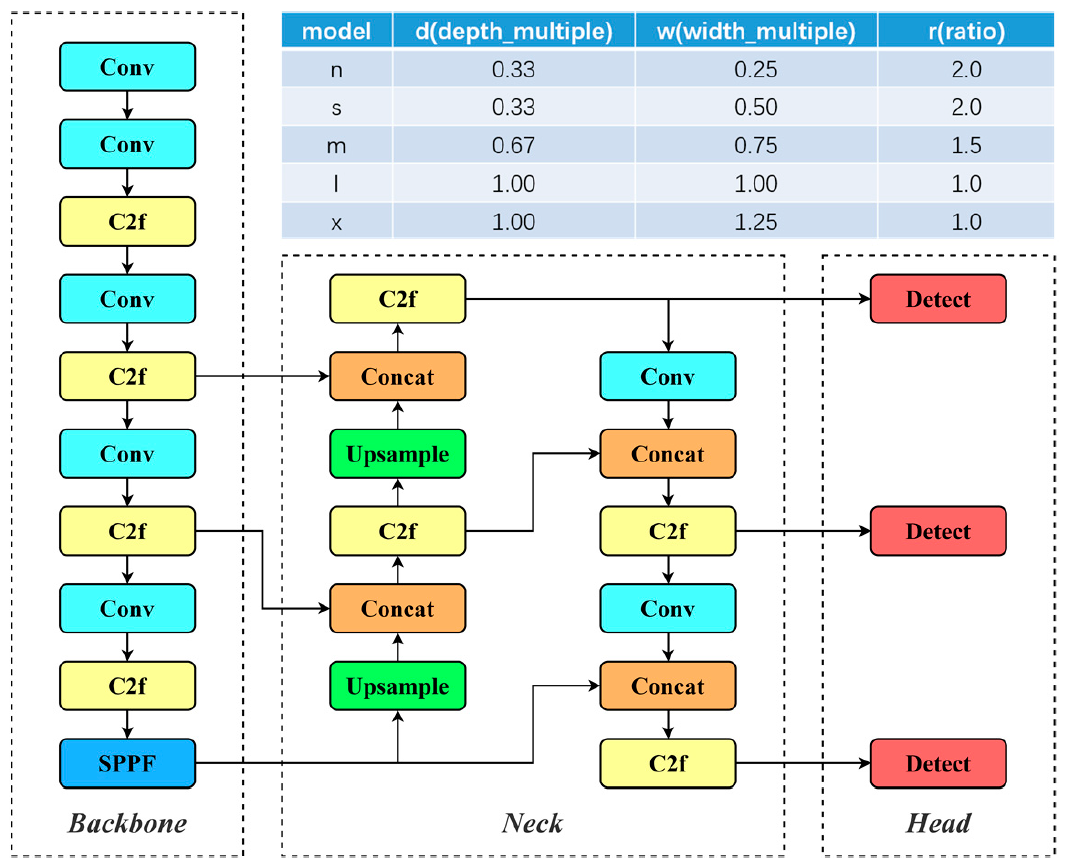
\includegraphics[width=.95\linewidth]{arsitektur_yolov8_standar.png}
\caption[Arsitektur dasar YOLOv8.]{Arsitektur dasar YOLOv8, digunakan kembali dari proposal; sumber Li dkk.~\cite{Li2024}.}
\label{fig:yolo-konseptual}
\end{figure}
Gambar~\ref{fig:yolo-konseptual} menunjukkan hubungan komponen YOLOv8 dan pilihan penskalaan jaringannya. Gambar ini digunakan untuk membedakan lokasi perubahan arsitektur pada ekstraksi fitur, penggabungan fitur, dan kepala deteksi.

\textit{Non-maximum suppression} (NMS) digunakan pada detektor yang memerlukan penyaringan kotak bertumpang tindih. Proses ini mempertimbangkan nilai kepercayaan dan tumpang tindih spasial. Ambang NMS memiliki fungsi berbeda dari ambang pencocokan prediksi dengan anotasi pada evaluasi. Perbedaan ini perlu dijaga agar aturan pascapemrosesan tidak tertukar dengan definisi keberhasilan deteksi.

\subsection{Varian pembanding}
YOLOv8n digunakan sebagai model dasar. YOLOv12n mewakili rancangan berbasis atensi yang dibahas oleh Tian dkk.~\cite{tian2025yolov12_primary}. YOLO26n menjadi pembanding lain dengan jalur deteksi \textit{end-to-end} yang berbeda~\cite{sapkota2025yolo26_primary}. Perbedaan tersebut berarti seluruh model tidak harus menggunakan langkah pascapemrosesan yang sama.

YOLOv8-PD dan YOLO-RD mewakili modifikasi yang dikembangkan untuk deteksi kerusakan jalan~\cite{Zeng2024,Wang2025}. Kedua model diterapkan melalui rekonstruksi lokal. Dengan demikian, pembanding penelitian adalah implementasi yang digunakan, bukan hasil reproduksi identik perangkat lunak penulis asli. Penskalaan nano pada model-model tersebut juga tidak menjamin kesamaan kapasitas jaringan.

\section{Modifikasi Arsitektur dan Pembobotan Kelas}
\subsection{Konvolusi ringan dan mekanisme atensi}
Konvolusi ringan bertujuan mengurangi kebutuhan operasi atau parameter pada pembentukan fitur. GhostNet memanfaatkan sejumlah fitur dasar dan transformasi yang lebih murah untuk menghasilkan fitur tambahan~\cite{han2020ghostnet}. Gagasan tersebut menjadi salah satu dasar penggunaan blok berbasis Ghost dalam model ringan. Efisiensi aktualnya tetap bergantung pada susunan jaringan dan perangkat eksekusi.

Mekanisme atensi mengatur kontribusi fitur secara adaptif. Dalam penelitian kerusakan jalan, atensi digunakan untuk membantu pengolahan informasi objek di antara tekstur latar yang kompleks~\cite{Li2024,Zeng2024}. Penerapan modul atensi tidak selalu mengurangi kebutuhan komputasi. Manfaat yang dilaporkan pada suatu penelitian juga tidak dapat langsung dipindahkan ke dataset atau implementasi lain.

YOLOv8-PD menggabungkan komponen berbasis Ghost, pengolahan atensi, dan kepala deteksi dengan berbagi konvolusi~\cite{Zeng2024}. YOLO-RD menggunakan modul operasi bintang, penyempurnaan atensi, dan pengolahan berbasis wavelet~\cite{Wang2025}. Komponen ini menjadi dasar rekonstruksi dalam penelitian. Penjelasan perbedaan rekonstruksi dan konfigurasi aktual ditempatkan pada Bab~\ref{bab:perancangan-sistem}.

\subsection{Ketimpangan kelas dan jumlah efektif sampel}
Ketimpangan kelas terjadi ketika frekuensi kategori pada data pelatihan tidak seimbang. Pembobotan kelas merupakan salah satu pendekatan untuk mengubah kontribusi kategori terhadap fungsi kerugian. Cui dkk. merumuskan jumlah efektif sampel berdasarkan gagasan bahwa tambahan informasi tidak selalu bertambah secara linear terhadap jumlah sampel~\cite{cui2019class}.

Jumlah efektif kelas $c$ dituliskan pada Persamaan~\eqref{eq:effective-number}.
\begin{equation}
E_c=\frac{1-\beta^{n_c}}{1-\beta}.
\label{eq:effective-number}
\end{equation}
Pada Persamaan~\eqref{eq:effective-number}, $n_c$ menyatakan jumlah sampel kelas $c$ dan $\beta$ berada pada rentang $0\leq\beta<1$. Penelitian ini mengoperasionalkan $n_c$ sebagai jumlah anotasi objek pada data latih. Kebalikan $E_c$ menjadi dasar bobot kelas. Normalisasi yang diterapkan dalam implementasi dirumuskan pada Persamaan~\eqref{eq:class-weight}.
\begin{equation}
a_c=\frac{1-\beta}{1-\beta^{n_c}},\qquad
w_c=\frac{K a_c}{\sum_{j=1}^{K}a_j}.
\label{eq:class-weight}
\end{equation}
Persamaan~\eqref{eq:class-weight} menghasilkan bobot $w_c$ dengan rata-rata satu untuk $K$ kelas pelatihan. Bobot dihitung hanya dari data latih. Pemisahan ini mencegah penggunaan frekuensi target untuk menentukan kontribusi kelas selama pelatihan sumber.

\subsection{Penerapan pada komponen klasifikasi}
Pembobotan tersebut diterapkan pada komponen \textit{binary cross-entropy} (BCE) untuk klasifikasi. Secara konseptual, bentuk berbobotnya dinyatakan pada Persamaan~\eqref{eq:weighted-bce}.
\begin{equation}
\ell_{ic}=-w_c\left[y_{ic}\log p_{ic}+(1-y_{ic})\log(1-p_{ic})\right].
\label{eq:weighted-bce}
\end{equation}
Pada Persamaan~\eqref{eq:weighted-bce}, $p_{ic}$ adalah probabilitas prediksi kelas $c$ pada posisi prediksi $i$. Simbol $y_{ic}$ menyatakan target klasifikasi, yang dapat berupa skor hasil penugasan target detektor. Persamaan ini menjelaskan kontribusi bobot pada klasifikasi; agregasi, normalisasi, dan komponen regresi mengikuti implementasi detektor.

Intervensi pada penelitian ini menggunakan $\beta=0{,}999$. Pembobotan berbasis frekuensi tersebut berbeda dari penambahan faktor modulasi berdasarkan kesulitan prediksi pada \textit{Focal Loss}. Karena eksperimen utama memakai pembobotan yang sama, hasilnya tidak digunakan untuk mengklaim keunggulan pembobotan atas fungsi kerugian lain. Klaim demikian memerlukan perbandingan khusus yang mengisolasi perubahan fungsi kerugian.

\section{Generalisasi dan Evaluasi Deteksi}
\subsection{Domain sumber, target, dan pengujian zero-shot}
Domain sumber adalah distribusi data yang digunakan untuk melatih model, sedangkan domain target merupakan lingkungan evaluasi yang berbeda. Penelitian deteksi kerusakan lintas negara menunjukkan bahwa kinerja perlu diperiksa pada kondisi di luar data sumber~\cite{arya2021deep,Arya2024846}. Perbedaan distribusi dapat melibatkan tampilan citra maupun komposisi objek.

Dalam penelitian ini, \textit{zero-shot} berarti penerapan model terlatih pada domain target tanpa \textit{fine-tuning}. Istilah ini merujuk pada perpindahan domain untuk kategori yang telah dikenal selama pelatihan. Pengujian tersebut bukan deteksi kategori baru yang sama sekali tidak tersedia pada data sumber.

Perbandingan lintas domain harus menggunakan himpunan kelas yang sama. Jika sumber dirata-ratakan atas enam kelas dan target atas lima kelas, selisih metrik turut dipengaruhi oleh perbedaan kategori. Penelitian ini karena itu memisahkan hasil enam kelas sumber dari perbandingan empat kelas kerusakan yang tersedia pada kedua domain. Selisih kinerja menjadi ukuran deskriptif pada dua himpunan data, tanpa mengidentifikasi penyebabnya secara kausal.

\subsection{Pencocokan kotak dan metrik deteksi}
\textit{Intersection over union} (IoU) mengukur tumpang tindih antara kotak prediksi $B_p$ dan kotak anotasi $B_g$~\cite{Li2024,Zeng2024}. Rumusnya ditunjukkan pada Persamaan~\eqref{eq:iou}.
\begin{equation}
\operatorname{IoU}(B_p,B_g)=\frac{|B_p\cap B_g|}{|B_p\cup B_g|}.
\label{eq:iou}
\end{equation}
Persamaan~\eqref{eq:iou} membandingkan luas irisan dengan luas gabungan kedua kotak. Nilainya digunakan untuk menentukan kecocokan spasial pada ambang tertentu. Untuk evaluasi per kelas, prediksi juga harus sesuai dengan kategori anotasi.

Prediksi yang cocok secara kelas dan lokasi disebut \textit{true positive} (TP). Prediksi yang tidak memperoleh pasangan valid dihitung sebagai \textit{false positive} (FP), sedangkan anotasi yang tidak terdeteksi menjadi \textit{false negative} (FN). Pencocokan membatasi penggunaan pasangan sehingga beberapa prediksi pada objek yang sama tidak semuanya dihitung benar. Berdasarkan hitungan tersebut, presisi dan \textit{recall} dirumuskan pada Persamaan~\eqref{eq:pr}.
\begin{equation}
P=\frac{TP}{TP+FP},\qquad R=\frac{TP}{TP+FN}.
\label{eq:pr}
\end{equation}
Persamaan~\eqref{eq:pr} membedakan ketepatan prediksi positif ($P$) dari kemampuan menemukan objek beranotasi ($R$). Keduanya berubah mengikuti ambang kepercayaan yang digunakan. F1 menyatukan kedua ukuran melalui rata-rata harmonis, seperti pada Persamaan~\eqref{eq:f1}.
\begin{equation}
F1_c=\frac{2P_cR_c}{P_c+R_c},\qquad
F1_{\mathrm{macro}}=\frac{1}{K}\sum_{c=1}^{K}F1_c.
\label{eq:f1}
\end{equation}
Pada Persamaan~\eqref{eq:f1}, $K$ adalah jumlah kelas yang dievaluasi. F1 bernilai nol ketika jumlah presisi dan \textit{recall} nol. Rata-rata makro memberikan kontribusi yang sama kepada setiap kelas, sehingga tidak didominasi langsung oleh kelas dengan anotasi terbanyak.

\textit{Average precision} (AP) merangkum kurva presisi--\textit{recall} ketika ambang kepercayaan berubah. Rata-rata AP antarkelas menghasilkan mAP~\cite{Li2024,Wu2023}, sebagaimana Persamaan~\eqref{eq:map}.
\begin{equation}
\operatorname{mAP}_{K}=\frac{1}{K}\sum_{c=1}^{K}AP_c.
\label{eq:map}
\end{equation}
Persamaan~\eqref{eq:map} digunakan dengan himpunan kelas yang dinyatakan secara eksplisit. mAP@0,5 menggunakan ambang IoU 0,5. mAP@0,5:0,95 merata-ratakan AP pada sepuluh ambang IoU dari 0,5 sampai 0,95 dengan langkah 0,05. Metrik kedua mempertimbangkan tuntutan ketepatan lokasi yang lebih beragam.

\subsection{Ukuran efisiensi komputasi}
Jumlah parameter menggambarkan banyaknya parameter dalam representasi model yang dihitung. GFLOPs menyatakan perkiraan miliaran operasi titik mengambang untuk satu komputasi maju pada ukuran masukan tertentu. GFLOPs bukan jumlah operasi per detik. Ukuran ini perlu dibedakan dari kecepatan aktual karena jenis operasi dan implementasi perangkat lunak turut berpengaruh~\cite{Wu2023}.

FPS menyatakan banyaknya citra yang dapat diproses per detik menurut prosedur pengukuran. Dalam penelitian ini, FPS diestimasi dari jumlah rerata waktu prapemrosesan, inferensi, dan pascapemrosesan per citra. Metrik tersebut tidak mencakup seluruh alur aplikasi, seperti akuisisi video dan penyajian antarmuka. Karena itu, FPS digunakan sebagai pembanding pada lingkungan uji yang tercatat.

\section{Penelitian Terkait dan Posisi Penelitian}
Penelitian terdahulu menyediakan dasar pemilihan model serta pertanyaan evaluasi. RDD-YOLO membahas pengembangan YOLOv8 dengan SimAM dan GhostConv~\cite{Li2024}. YOLOv8-PD menekankan rancangan ringan berbasis YOLOv8n~\cite{Zeng2024}, sedangkan YOLO-RD mengembangkan pemrosesan fitur untuk deteksi kerusakan~\cite{Wang2025}. Ketiganya menjadi rujukan untuk menilai ketepatan dan kebutuhan komputasi secara bersama.

Kajian Matouq dkk. memberi dasar untuk memperhatikan kategori penutup saluran dan tambalan dalam deteksi lubang~\cite{matouq2024ai}. Sementara itu, penelitian Hugo dkk. menggunakan citra jalan Indonesia untuk mengevaluasi EfficientDet~\cite{hugo2025efficientdet}. Penelitian tersebut mendukung kebutuhan evaluasi lokal, tetapi protokolnya berbeda dari transfer tanpa pelatihan ulang yang digunakan di sini. Ringkasan keterkaitannya disajikan pada Tabel~\ref{tab:penelitian-terkait}.

\begin{table}[H]
\centering
\caption{Penelitian terkait dan keterkaitannya dengan penelitian ini.}
\label{tab:penelitian-terkait}
\begingroup\fontsize{10}{13}\selectfont
\begin{tabularx}{\linewidth}{|p{2.5cm}|X|X|}\hline
\rowcolor{black}\HeaderTabel{Penelitian}&\HeaderTabel{Fokus}&\HeaderTabel{Keterkaitan}\\\hline
Li dkk.~\cite{Li2024} & RDD-YOLO pada RDD2022; atensi dan konvolusi ringan & Dasar pembahasan modifikasi YOLO untuk citra jalan\\\hline
Zeng dan Zhong~\cite{Zeng2024} & YOLOv8-PD untuk deteksi kerusakan jalan & Dasar rekonstruksi model berorientasi efisiensi\\\hline
Wang dkk.~\cite{Wang2025} & YOLO-RD dengan pengembangan ekstraksi fitur & Dasar rekonstruksi model pembanding\\\hline
Matouq dkk.~\cite{matouq2024ai} & Deteksi lubang beserta objek permukaan terkait & Motivasi pengujian label pengecoh\\\hline
Hugo dkk.~\cite{hugo2025efficientdet} & EfficientDet pada citra jalan Indonesia & Konteks evaluasi pada data lokal\\\hline
Arya dkk.~\cite{arya2021deep,Arya2024846} & Dataset dan evaluasi lintas negara & Dasar pengujian generalisasi antardomain\\\hline
\end{tabularx}\endgroup
\end{table}
Tabel~\ref{tab:penelitian-terkait} menghubungkan literatur dengan keputusan penelitian, tanpa menjadikan skor dari dataset berbeda sebagai peringkat langsung. Perbandingan dalam TA ini menggunakan data sumber yang sama, implementasi yang terdokumentasi, dan evaluasi target tanpa penyesuaian bobot.

Posisi penelitian adalah evaluasi bersama terhadap model dasar, model berbasis pengembangan arsitektur, dan rekonstruksi model khusus kerusakan jalan. Pengujian label pengecoh melengkapi perbandingan tersebut. Kontribusinya terletak pada karakterisasi kinerja implementasi dan generalisasi pada target lokal, bukan pada klaim penemuan arsitektur baru atau keunggulan universal suatu model.

\chapter{PERANCANGAN SISTEM}
\label{bab:perancangan-sistem}

Bab ini menjelaskan pelaksanaan penelitian berdasarkan data, implementasi, dan konfigurasi eksperimen yang tersedia. Sistem yang dirancang merupakan alur eksperimen deteksi objek. Masukannya adalah citra jalan dan anotasi, sedangkan keluarannya berupa model terlatih, prediksi, serta metrik evaluasi.

\section{Desain Perancangan Sistem}
Penelitian menggunakan desain komparatif dengan tiga fokus yang mengikuti rumusan masalah. Fokus pertama adalah kinerja deteksi pada domain sumber beserta perbandingan penggunaan kelas pengecoh. Fokus kedua adalah keseimbangan ketepatan dan kebutuhan komputasi. Fokus ketiga adalah kemampuan generalisasi pada citra jalan Indonesia tanpa pelatihan ulang.

Lima model dibandingkan pada pembagian data sumber yang sama. Data latih digunakan untuk pembaruan parameter dan perhitungan bobot kelas. Data validasi digunakan untuk pemantauan, penghentian dini, dan pemilihan \textit{checkpoint}. Data uji sumber digunakan untuk pelaporan kinerja akhir. Data target digunakan hanya untuk pengujian lintas domain, tanpa pembaruan bobot model.

Rancangan mempertahankan tujuan proposal, dengan beberapa penyesuaian sesuai pelaksanaan. Model modifikasi direalisasikan sebagai rekonstruksi YOLOv8-PD dan YOLO-RD. Penanganan ketimpangan menggunakan pembobotan jumlah efektif sampel. Pengujian target mencakup seluruh model, sehingga peringkat sumber dan target dapat diperiksa bersama. Jumlah data target yang dievaluasi adalah 307 citra, berbeda dari target pengumpulan minimal 500 citra pada proposal.

\section{Diagram Blok}
Alur pemrosesan sumber dan target ditunjukkan pada Gambar~\ref{fig:alur-penelitian}. Jalur target menggunakan model yang telah dipilih melalui validasi sumber.
\begin{figure}[H]
\centering
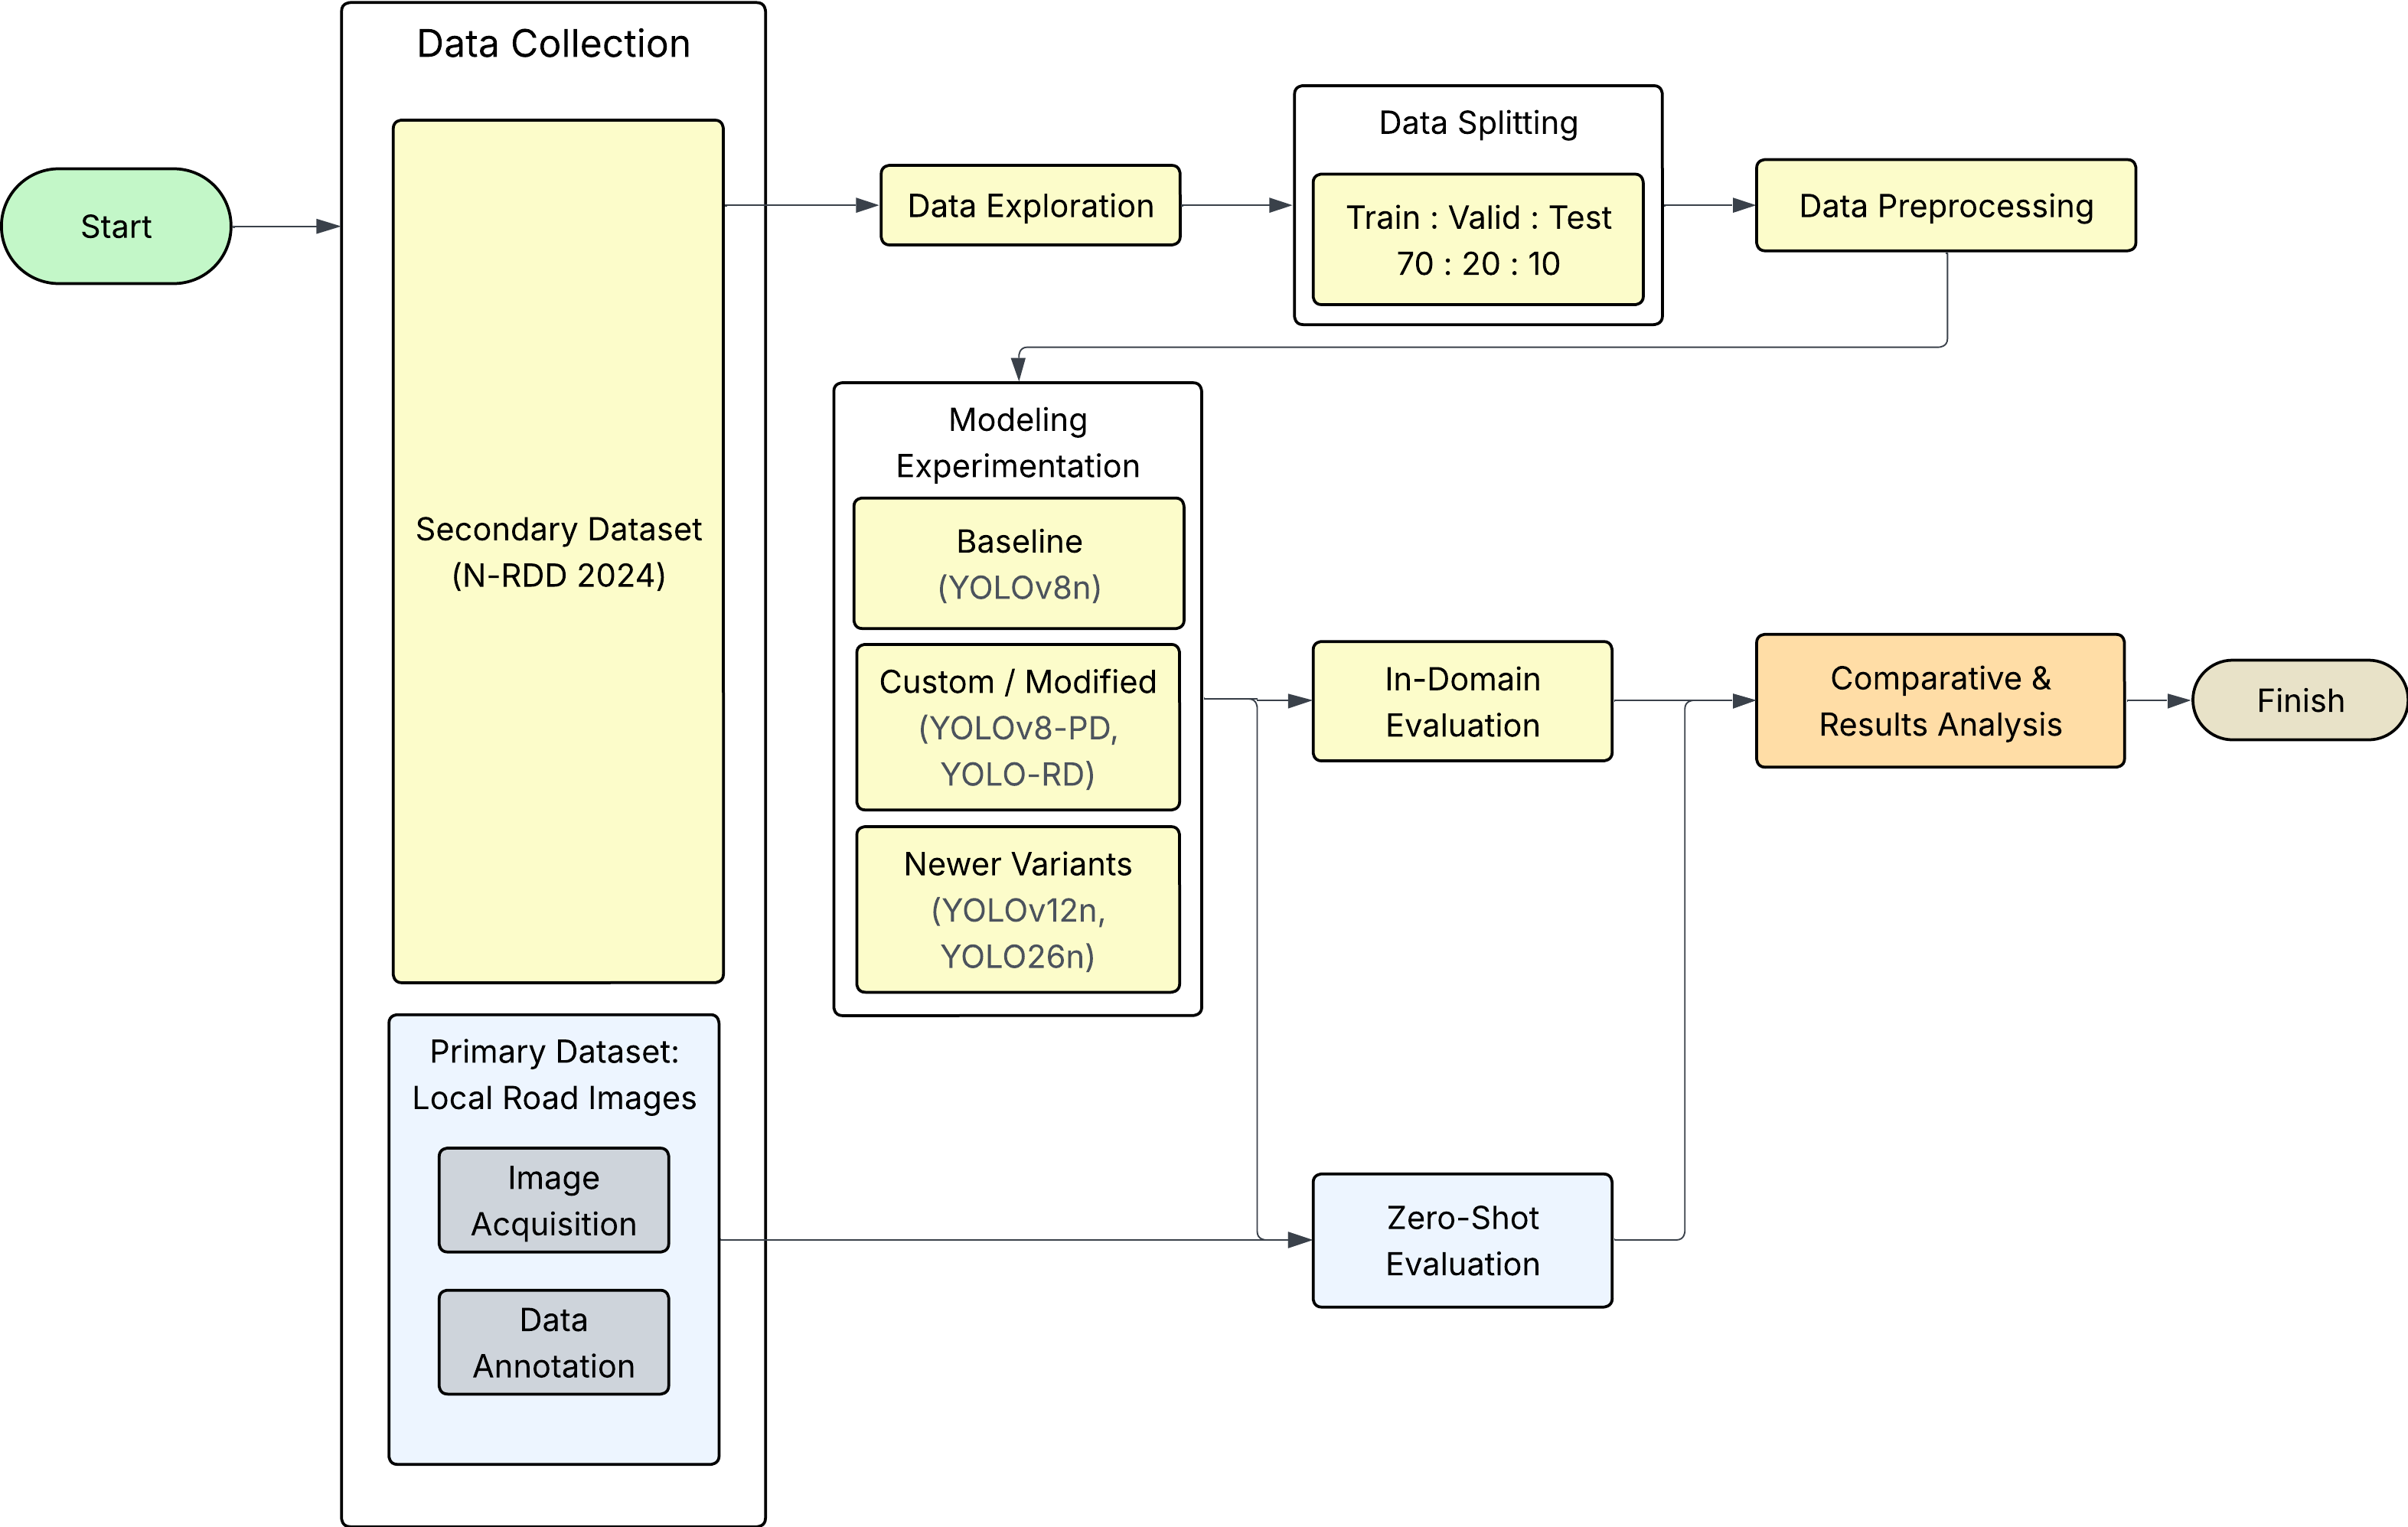
\includegraphics[width=\linewidth]{methodology_workflow.png}
\caption{Alur eksperimen komparatif dan pengujian lintas domain.}
\label{fig:alur-penelitian}
\end{figure}
Gambar~\ref{fig:alur-penelitian} membedakan jalur data sekunder untuk pelatihan dari data primer untuk evaluasi \textit{zero-shot}. Pada jalur data primer, akuisisi diikuti anotasi sebelum evaluasi. Jalur pemodelan memasok bobot terbaik berdasarkan validasi sumber, tanpa pembaruan bobot pada target. Kelompok \textit{custom/modified} pada diagram merujuk pada rekonstruksi YOLOv8-PD dan YOLO-RD. Rasio 70:20:10 merupakan proporsi rencana; jumlah aktual dijelaskan pada bagian pembagian data.

Evaluasi sumber mencakup ketepatan deteksi dan efisiensi komputasi. Eksperimen empat kelas menjadi analisis tambahan pada domain sumber, sedangkan pengujian target menggunakan bobot pelatihan utama enam kelas. Perbandingan lintas domain dirangkum pada empat kelas kerusakan yang sama.

\section{Fungsi dan Fitur}
Alur eksperimen menyediakan fungsi penyiapan data, pelatihan, evaluasi, dan pemeriksaan prediksi. Penyiapan data mencakup penyaringan kelas serta penyelarasan identitas kategori. Pelatihan menghasilkan bobot setiap model dengan pencatatan argumen dan perkembangan metrik. Evaluasi menghasilkan metrik agregat, metrik per kelas, serta ringkasan waktu pemrosesan.

Pemeriksaan prediksi digunakan untuk membaca contoh deteksi benar, objek terlewat, dan prediksi yang tidak sesuai anotasi. Analisis tambahan membandingkan pelatihan empat dan enam kelas serta menghitung prediksi lubang yang bertumpang tindih dengan anotasi pengecoh. Keluaran tersebut mendukung interpretasi hasil, tetapi contoh visual tidak diperlakukan sebagai ukuran frekuensi kesalahan seluruh dataset.

\section{Desain Perangkat Keras dan Lunak}
Implementasi menggunakan Python, PyTorch, dan kerangka Ultralytics. Model rekonstruksi menggunakan modul tambahan yang didaftarkan pada pemuat arsitektur Ultralytics. Anotasi target dikelola menggunakan Roboflow. Lingkungan pengukuran kecepatan sumber dirangkum pada Tabel~\ref{tab:lingkungan}.
\begin{table}[H]
\centering
\caption{Lingkungan evaluasi untuk pengukuran kecepatan sumber.}
\label{tab:lingkungan}
\begin{tabularx}{\linewidth}{|l|X|}\hline
\rowcolor{black}\HeaderTabel{Komponen}&\HeaderTabel{Konfigurasi tercatat}\\\hline
GPU & NVIDIA GeForce RTX 4070 SUPER, memori 12 GB\\\hline
Python & 3.12.3\\\hline
PyTorch dan CUDA & PyTorch 2.5.1; CUDA 12.1\\\hline
Ultralytics & 8.4.108\\\hline
Ukuran masukan & 640 piksel\\\hline
Data pengukuran & Data uji sumber, 995 citra\\\hline
\end{tabularx}
\end{table}
Tabel~\ref{tab:lingkungan} mengikuti log evaluasi sumber yang menjadi dasar estimasi FPS. Konfigurasi tersebut tidak digeneralisasi sebagai lingkungan seluruh eksperimen tambahan. Penghitungan ulang kompleksitas model menggunakan Ultralytics 8.4.177 dan dipisahkan dari pengukuran waktu yang tercatat pada versi 8.4.108.

\section{Data dan Prapemrosesan}
\subsection{Akuisisi dan seleksi data sumber}
Data sekunder berasal dari N-RDD2024~\cite{kaya2024nrdd2024}. Sesuai eksplorasi pada proposal, subset Asia awal berjumlah 10.395 citra. Penyaringan mempertahankan citra yang memiliki sedikitnya satu objek dari enam kelas penelitian dan menghasilkan 9.670 citra. Anotasi di luar kategori tersebut tidak digunakan dalam pelatihan.

Distribusi citra sumber terdiri atas 6.638 citra Jepang, 1.977 citra Tiongkok, dan 1.055 citra India. Proporsinya ditunjukkan pada Gambar~\ref{fig:distribusi-negara}.
\begin{figure}[H]
\centering
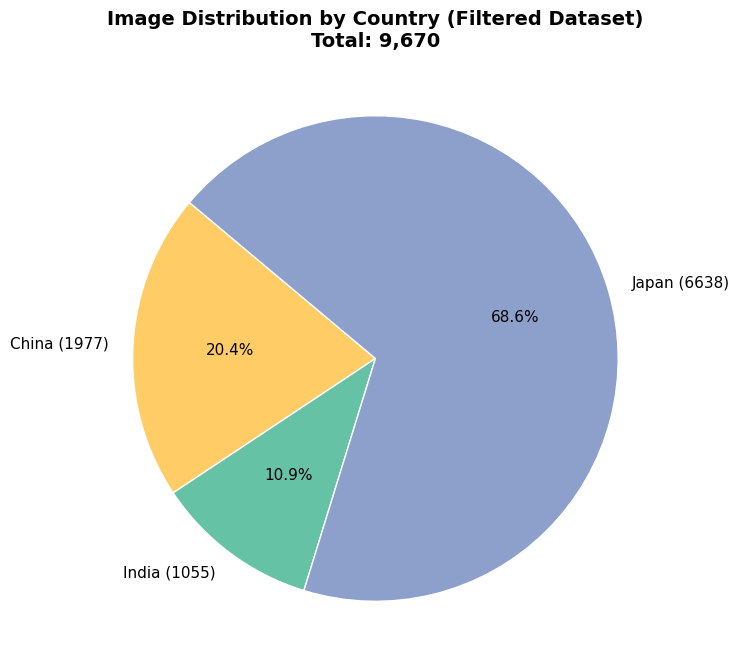
\includegraphics[width=.76\linewidth]{distribusi_gambar.png}
\caption{Distribusi citra sumber menurut negara, digunakan kembali dari eksplorasi data proposal.}
\label{fig:distribusi-negara}
\end{figure}
Gambar~\ref{fig:distribusi-negara} memperlihatkan bahwa kontribusi jumlah citra ketiga negara tidak sama. Komposisi ini perlu dipertimbangkan saat membaca hasil agregat. Proporsi citra bukan ukuran kesamaan karakteristik jalan suatu negara dengan Indonesia.

Contoh anotasi enam kelas disajikan pada Gambar~\ref{fig:contoh-kelas}. Setiap panel memperlihatkan contoh kategori, bukan hasil prediksi model.
\begin{figure}[H]
\centering
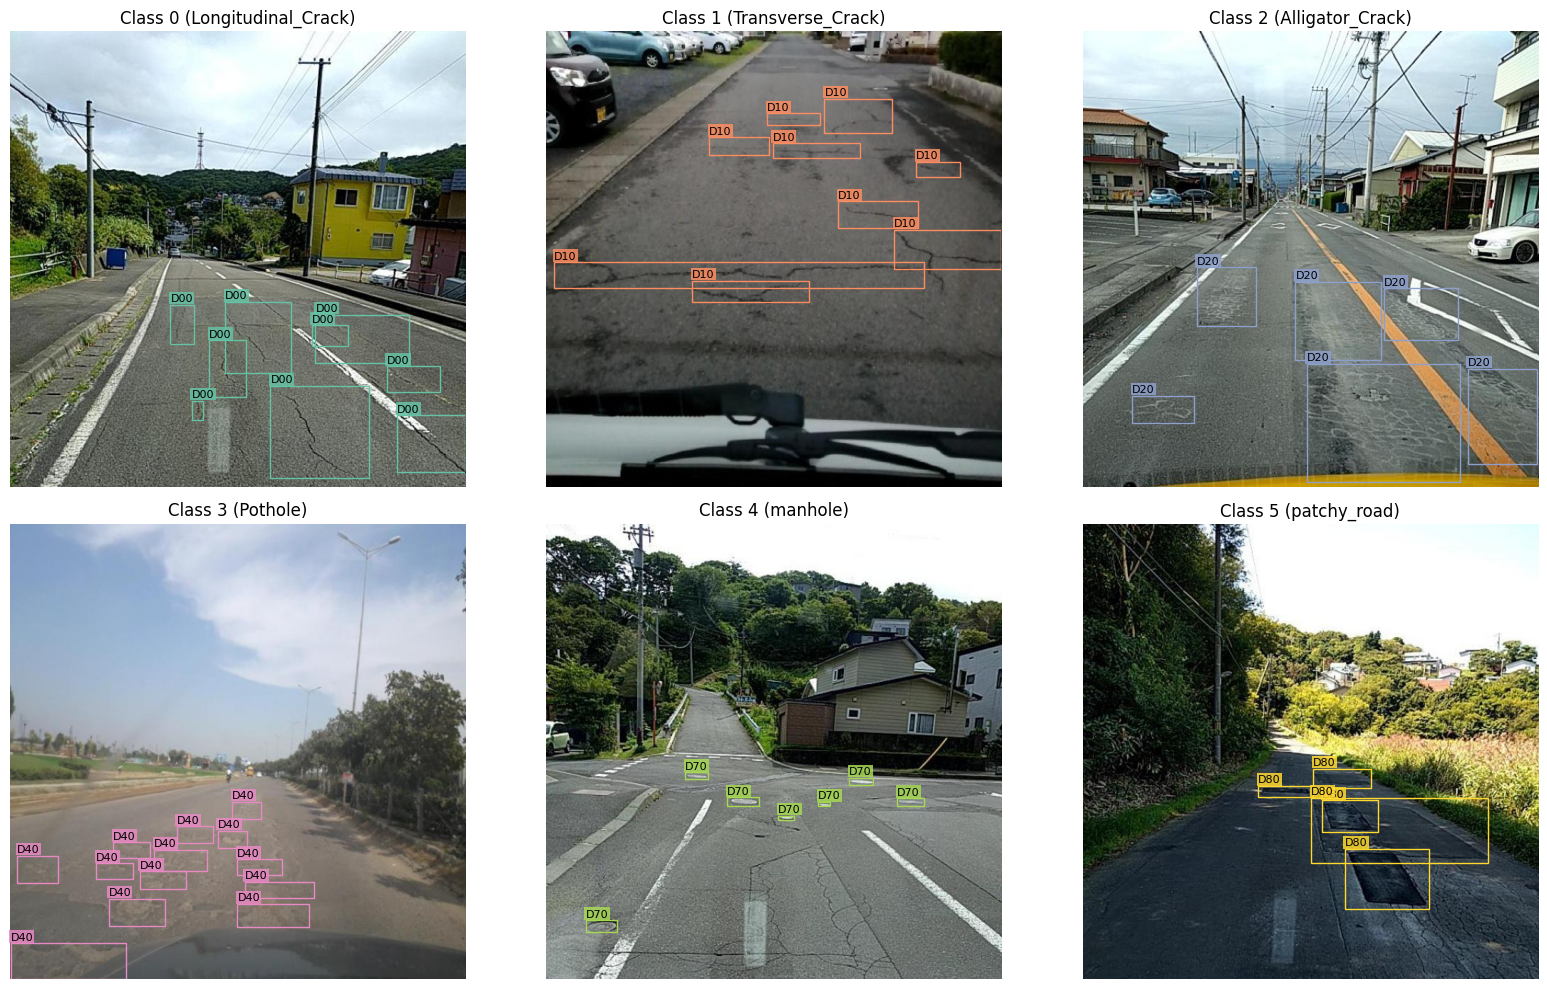
\includegraphics[width=\linewidth]{object_sample.png}
\caption{Contoh anotasi enam kelas pada data sumber, digunakan kembali dari proposal.}
\label{fig:contoh-kelas}
\end{figure}
Gambar~\ref{fig:contoh-kelas} memperlihatkan keragaman bentuk, ukuran, dan lokasi kotak pembatas. Visualisasi ini membantu menjelaskan objek yang menjadi masukan pelatihan. Panel yang dipilih tidak dimaksudkan untuk menyatakan distribusi kesulitan seluruh citra.

\subsection{Pembagian data dan distribusi anotasi}
Pembagian data sumber mengikuti rancangan sekitar 70:20:10 dengan stratifikasi multilabel untuk menjaga kemiripan proporsi kelas. Jumlah aktual citra pada setiap bagian disajikan pada Tabel~\ref{tab:pembagian}. Angka aktual digunakan sebagai dasar deskripsi eksperimen, bukan hasil pembulatan rasio rencana.
\begin{table}[H]
\centering
\caption{Inventaris pembagian citra dan anotasi sumber.}
\label{tab:pembagian}
\begingroup\fontsize{10}{13}\selectfont
\begin{tabularx}{\linewidth}{|X|r|r|r|}\hline
\rowcolor{black}\HeaderTabel{Bagian}&\HeaderTabel{Citra}&\HeaderTabel{Anotasi 6 kelas}&\HeaderTabel{Anotasi 4 kelas}\\\hline
Latih & 6.777 & 17.092 & 14.351\\\hline
Validasi & 1.898 & 4.773 & 3.996\\\hline
Uji & 995 & 2.425 & 2.035\\\hline
Total & 9.670 & 24.290 & 20.382\\\hline
\end{tabularx}\endgroup
\end{table}
Tabel~\ref{tab:pembagian} membedakan jumlah citra dari jumlah anotasi sebelum pemuatan validator. Log validasi mencatat penghapusan satu anotasi penutup saluran yang duplikat, sehingga evaluasi menggunakan 4.772 objek validasi. Perbedaan tersebut tidak mengubah inventaris 4.773 baris label atau jumlah 2.425 objek uji.

Distribusi kelas pada tiap bagian disajikan pada Tabel~\ref{tab:distribusi-kelas}.
\begin{table}[H]
\centering
\caption{Jumlah anotasi per kelas pada inventaris sumber.}
\label{tab:distribusi-kelas}
\begingroup\fontsize{10}{13}\selectfont
\begin{tabularx}{\linewidth}{|X|r|r|r|}\hline
\rowcolor{black}\HeaderTabel{Kelas}&\HeaderTabel{Latih}&\HeaderTabel{Validasi}&\HeaderTabel{Uji}\\\hline
Retak memanjang &4.555&1.257&635\\\hline
Retak melintang &3.219&897&446\\\hline
Retak buaya &4.385&1.245&642\\\hline
Lubang jalan &2.192&597&312\\\hline
Penutup saluran &2.270&645&321\\\hline
Jalan bertambal &471&132&69\\\hline
\end{tabularx}\endgroup
\end{table}
Tabel~\ref{tab:distribusi-kelas} memperlihatkan ketimpangan yang menjadi dasar pembobotan kelas. Pada data latih, rasio jumlah retak memanjang terhadap jalan bertambal sekitar 9,67. Bobot dihitung dari kolom latih saja menggunakan Persamaan~\eqref{eq:class-weight}, sehingga distribusi validasi, uji, dan target tidak menentukan pembobotan.

\subsection{Akuisisi dan anotasi data target}
Data primer diperoleh melalui perekaman menggunakan ponsel Android yang diarahkan ke jalan pada resolusi 1080p. Pengambilan dilakukan pada kedua arah perjalanan, terutama di Jalan Raya Bojongsoang serta jalan sekitarnya di Kabupaten Bandung. Video disampel pada interval satu bingkai per detik. Citra terpilih dianotasi oleh satu anotator menggunakan Roboflow dan dipotong pada bagian tengah menjadi $640\times640$ piksel.

Ekspor yang digunakan tersimpan sebagai RDD-indo-v4 dan memuat 307 citra pada bagian bernama \texttt{valid}. Metadata lokal mencatat proyek \texttt{rdd-indo-crop} versi 4. Dalam eksperimen ini, bagian tersebut digunakan sebagai data uji target. Nama \texttt{valid} dari ekspor tidak berarti bahwa data Indonesia digunakan untuk memilih bobot model.

Inventaris target berisi 502 anotasi, dengan 39 citra tanpa anotasi objek. Empat kelas kerusakan mencakup 481 anotasi, sedangkan jalan bertambal mencakup 21 anotasi. Tidak terdapat anotasi penutup saluran. Pemetaan kategori target ke identitas kelas sumber ditunjukkan pada Tabel~\ref{tab:pemetaan-target}.
\begin{table}[H]
\centering
\caption{Pemetaan kelas target dan jumlah anotasinya.}
\label{tab:pemetaan-target}
\begingroup\fontsize{10}{13}\selectfont
\begin{tabularx}{\linewidth}{|c|X|c|r|}\hline
\rowcolor{black}\HeaderTabel{ID target}&\HeaderTabel{Kategori}&\HeaderTabel{ID sumber}&\HeaderTabel{Anotasi}\\\hline
0 & Retak buaya &2&48\\\hline
1 & Retak memanjang &0&231\\\hline
2 & Jalan bertambal &5&21\\\hline
3 & Lubang jalan &3&70\\\hline
4 & Retak melintang &1&132\\\hline
\end{tabularx}\endgroup
\end{table}
Tabel~\ref{tab:pemetaan-target} memastikan bahwa perbedaan urutan label tidak mengubah makna kelas saat evaluasi. Seluruh 307 citra dipertahankan, termasuk citra tanpa anotasi. Kelas tanpa anotasi tidak diberi AP nol sebagai pengganti hasil evaluasi yang tidak tersedia.

Tambalan yang aus atau berbatas tidak teratur tetap termasuk kategori jalan bertambal pada anotasi target. Keterbatasan anotasi oleh satu orang dan cakupan lokasi perlu dipertimbangkan dalam interpretasi. Data ini digunakan sebagai pengujian lokal, bukan sampel yang mewakili seluruh jalan Indonesia.

\subsection{Representasi data dan augmentasi}
Anotasi menggunakan format YOLO yang memuat identitas kelas dan koordinat kotak ternormalisasi. Ukuran masukan model ditetapkan 640 piksel. Normalisasi intensitas dan penyesuaian masukan mengikuti pemuat data Ultralytics. Augmentasi hanya diterapkan pada pelatihan untuk membentuk variasi masukan.

Augmentasi utama mencakup Mosaic, MixUp, pembalikan horizontal, translasi, dan perubahan skala. Mosaic menggabungkan beberapa citra dalam satu masukan, sedangkan MixUp mencampurkan pasangan citra. Nilai konfigurasi aktual dicantumkan pada bagian pelatihan. Data uji digunakan tanpa augmentasi pelatihan agar evaluasi mengacu pada citra yang ditetapkan.

\section{Implementasi Model dan Pelatihan}
\subsection{Model bawaan dan rekonstruksi}
YOLOv8n, YOLOv12n, dan YOLO26n dimuat dari model bawaan dengan bobot pralatih. YOLOv8-PD dan YOLO-RD dibangun melalui definisi arsitektur lokal berdasarkan publikasi rujukan~\cite{Zeng2024,Wang2025}. Bobot YOLOv8n yang kompatibel dimuat ke kedua model rekonstruksi. Proses ini merupakan transfer parsial, bukan inisialisasi identik untuk seluruh parameter.

Rekonstruksi YOLOv8-PD mempertahankan struktur dasar ekstraksi fitur YOLOv8 dan menambahkan BoT serta LSKA setelah SPPF. Bagian penggabungan fitur menggunakan C2fGhost dan LSKA. Kepala deteksi menggunakan LSCDHead. Susunan ini merupakan implementasi lokal dari elemen rancangan YOLOv8-PD.

Rekonstruksi YOLO-RD menggunakan modul SOM pada \textit{backbone}, ARM pada fitur beberapa tingkat, serta WTHead dengan konvolusi berbasis wavelet. Fusi tambahan direalisasikan melalui \textit{upsample}, konkatenasi, dan konvolusi $1\times1$. Realisasi tersebut berbeda dari penjumlahan berbobot pada formulasi MAF asli~\cite{Wang2025}. Perbedaan ini membatasi klaim kesetaraan dengan model publikasi.

Kedua rekonstruksi memakai pengali kedalaman 0,33 dan lebar 0,25 pada skala nano. Namun, modul tambahan tetap menghasilkan jumlah parameter yang berbeda. Perbandingan karena itu menilai implementasi lengkap, bukan pengaruh topologi dengan kapasitas yang sepenuhnya dikendalikan.

\subsection{Konfigurasi pelatihan}
Argumen pelatihan setiap eksperimen disimpan bersama bobot model. Konfigurasi bersama pada pelatihan utama disajikan pada Tabel~\ref{tab:konfigurasi-latih}.
\begin{table}[H]
\centering
\caption{Konfigurasi pelatihan utama enam kelas.}
\label{tab:konfigurasi-latih}
\begingroup\fontsize{10}{13}\selectfont
\begin{tabularx}{\linewidth}{|X|X|}\hline
\rowcolor{black}\HeaderTabel{Pengaturan}&\HeaderTabel{Nilai}\\\hline
Ukuran masukan; ukuran batch &640 piksel; 16\\\hline
Batas epoch; patience &300; 40\\\hline
Seed; deterministic &42; aktif\\\hline
Optimizer &Pemilihan otomatis (\texttt{auto})\\\hline
Weight decay &0,0005\\\hline
Penjadwalan laju belajar &\textit{Cosine learning rate} aktif\\\hline
Mosaic; penutupan Mosaic &1,0; 10 epoch terakhir yang dijadwalkan\\\hline
MixUp; pembalikan horizontal &0,05; 0,5\\\hline
Translasi; perubahan skala &0,10; 0,50\\\hline
Rotasi &0 derajat\\\hline
Pembobotan kelas &Jumlah efektif sampel; $\beta=0{,}999$\\\hline
\end{tabularx}\endgroup
\end{table}
Tabel~\ref{tab:konfigurasi-latih} menyatakan argumen yang diberikan pada pelatihan, bukan jaminan bahwa semua model berhenti pada epoch yang sama. Pemilihan optimizer otomatis juga dapat menentukan pengaturan efektif yang berbeda. Nilai nominal laju belajar tidak diperlakukan sebagai bukti bahwa seluruh model menggunakan optimizer dan laju awal identik.

AMP diaktifkan pada ketiga model bawaan dan dinonaktifkan pada kedua rekonstruksi untuk pelatihan utama enam kelas. Pada eksperimen empat kelas, argumen yang tersimpan mencatat AMP aktif untuk kelima model. Perbedaan ini dicatat sebagai bagian konfigurasi perbandingan, sehingga ablasi tidak dinyatakan mengendalikan semua aspek pelatihan secara identik.

Bobot kelas dihitung dari frekuensi objek latih dan dinormalisasi menjadi rata-rata satu. Implementasi memasang bobot pada inisialisasi fungsi kerugian model agar tetap digunakan ketika pelatih membangun ulang model. Komponen klasifikasi menggunakan bobot tersebut, sementara jalur fungsi kerugian mengikuti arsitektur, termasuk jalur \textit{end-to-end} pada YOLO26n.

\subsection{Pemilihan bobot dan keterlacakan}
Bobot terbaik disimpan berdasarkan nilai \textit{fitness} validasi Ultralytics. Mekanisme penghentian dini menggunakan kesabaran 40 epoch. Pengujian sumber dan target memuat bobot terbaik dari proses ini. Tidak dilakukan pemilihan ulang \textit{checkpoint} berdasarkan skor target.

Artefak yang disimpan meliputi argumen pelatihan, riwayat metrik, bobot terbaik, serta hasil evaluasi per kelas. Konfigurasi tersimpan digunakan untuk mendeskripsikan pelaksanaan aktual. Hal ini diperlukan karena konstanta pada sel notebook yang telah diedit tidak selalu menggambarkan eksperimen sebelumnya.

\section{Protokol Pengujian dan Analisis}
\subsection{Evaluasi deteksi pada domain sumber}
Evaluasi akhir menggunakan 995 citra uji sumber. Metrik utama adalah mAP@0,5, dilengkapi mAP@0,5:0,95, presisi, \textit{recall}, dan F1. Hasil enam kelas menggambarkan tugas pelatihan utama. Rata-rata empat kelas kerusakan dilaporkan terpisah ketika digunakan untuk perbandingan antarkonfigurasi atau antardomain.

Evaluasi AP memakai ukuran masukan 640 piksel, ambang kepercayaan minimum 0,001, dan ambang IoU NMS 0,6 pada jalur yang menggunakan NMS. Ambang NMS tersebut bukan ambang IoU untuk menentukan TP. Penghitungan AP tetap menggunakan ambang pencocokan sesuai metrik yang dinyatakan.

F1 per kelas dihitung dari presisi dan \textit{recall} keluaran evaluator. Keluaran tersebut menggunakan ambang kepercayaan yang memaksimalkan kurva rerata F1 yang dihaluskan pada bagian data yang dievaluasi. Rata-rata makro dihitung menggunakan Persamaan~\eqref{eq:f1}. Dengan demikian, F1 ini merupakan ringkasan pada titik operasi hasil evaluasi, bukan kinerja pada ambang penerapan tetap yang dipilih sebelumnya.

\subsection{Evaluasi efisiensi}
Jumlah parameter dan GFLOPs dihitung dari \textit{checkpoint} akhir dalam bentuk model \textit{fused} pada masukan 640 piksel. Bentuk ini menggabungkan operasi tertentu untuk inferensi. Angkanya perlu dibedakan dari hitungan model sebelum penggabungan atau estimasi versi perangkat lunak lain.

Estimasi FPS menggunakan waktu rata-rata per citra yang dilaporkan validator. Perhitungannya dinyatakan pada Persamaan~\eqref{eq:fps}.
\begin{equation}
\operatorname{FPS}_{\mathrm{estimasi}}=\frac{1000}{t_{\mathrm{pra}}+t_{\mathrm{inferensi}}+t_{\mathrm{pasca}}}.
\label{eq:fps}
\end{equation}
Pada Persamaan~\eqref{eq:fps}, seluruh waktu menggunakan satuan milidetik per citra. Estimasi mencakup tiga tahap pemrosesan validator dan tidak berasal dari pengujian aplikasi terpisah. Pengukuran ini tidak mencakup percobaan khusus variasi batch atau protokol \textit{warm-up} mandiri.

Analisis efisiensi membandingkan ketepatan deteksi dengan parameter, GFLOPs, dan estimasi FPS. Pemilihan kandidat dibahas sesuai prioritas metrik, tanpa membentuk skor gabungan dengan bobot yang tidak ditetapkan dalam eksperimen. Kecepatan pada GPU pengujian tidak diproyeksikan langsung ke perangkat \textit{edge}.

\subsection{Perbandingan pelatihan empat dan enam kelas}
Eksperimen tambahan menghapus anotasi D70 dan D80 dari data sumber, dengan mempertahankan citra serta pembagian latih, validasi, dan uji. Citra yang menjadi tanpa anotasi tetap disertakan. Kelima arsitektur dilatih pada empat kelas kerusakan, dengan pembobotan yang dihitung kembali dari distribusi latih empat kelas.

Kinerja model empat kelas dibandingkan dengan model enam kelas pada D00, D10, D20, dan D40 saja. Prosedur ini menghindari perbandingan rata-rata atas himpunan kategori berbeda. Hasil dibaca sebagai perubahan yang teramati pada konfigurasi pelatihan, dengan memperhatikan perbedaan AMP dan sifat satu \textit{seed} eksperimen.

Analisis diagnostik tambahan menghitung kotak prediksi lubang dengan kepercayaan sedikitnya 0,25 yang bertumpang tindih dengan anotasi pengecoh pada IoU sedikitnya 0,5. Satu kotak prediksi dihitung sekali meskipun bertumpang tindih dengan beberapa anotasi. Sebaliknya, beberapa kotak prediksi dapat bertumpang tindih dengan objek yang sama. Hitungan ini bukan tingkat FP berbasis pencocokan unik antarobjek.

\subsection{Pengujian zero-shot pada target Indonesia}
Pengujian target menggunakan bobot enam kelas tanpa \textit{fine-tuning}, dengan pemetaan pada Tabel~\ref{tab:pemetaan-target}. Seluruh citra dipertahankan. Ambang kepercayaan minimum dan ukuran masukan mengikuti evaluasi sumber.

Perbandingan utama menggunakan mAP empat kelas kerusakan pada kedua domain. Penutup saluran dan jalan bertambal tidak masuk rata-rata tersebut. Evaluasi lima kelas yang menyertakan jalan bertambal diperlakukan sebagai analisis tambahan yang terpisah.

Penurunan absolut dan relatif dihitung melalui Persamaan~\eqref{eq:gap-absolut} dan~\eqref{eq:gap-relatif}.
\begin{equation}
\Delta_{\mathrm{abs}}=100\left(\operatorname{mAP}^{S}_{4}-\operatorname{mAP}^{T}_{4}\right).
\label{eq:gap-absolut}
\end{equation}
Persamaan~\eqref{eq:gap-absolut} menyatakan selisih dalam poin persentase ketika mAP sumber ($S$) dan target ($T$) ditulis pada skala nol sampai satu. Subskrip empat menegaskan bahwa kedua rata-rata menggunakan kategori yang sama.
\begin{equation}
\Delta_{\mathrm{rel}}=100\left(1-\frac{\operatorname{mAP}^{T}_{4}}{\operatorname{mAP}^{S}_{4}}\right)\%.
\label{eq:gap-relatif}
\end{equation}
Persamaan~\eqref{eq:gap-relatif} menyatakan penurunan sebagai persentase terhadap kinerja sumber, selama penyebut lebih besar dari nol. Kedua ukuran merangkum kesenjangan kinerja antardataset. Nilainya bukan ukuran langsung jarak distribusi atau bukti pengaruh kausal pencahayaan, tekstur, dan lokasi.

\subsection{Batas interpretasi}
Perbandingan satu \textit{seed} belum mengukur variasi antarulangan, sehingga selisih metrik tidak dinyatakan signifikan. Rekonstruksi, transfer parsial, dan perbedaan konfigurasi membatasi klaim pengaruh modul secara kausal. Cakupan target lokal dan anotasi oleh satu orang juga membatasi generalisasi. Contoh visual serta hitungan tumpang tindih digunakan sebagai bukti deskriptif.

\chapter{HASIL PERCOBAAN DAN ANALISIS}
\label{bab:hasil-percobaan-dan-analisis}

Bab ini menyajikan hasil pelaksanaan eksperimen yang dirancang pada Bab~\ref{bab:perancangan-sistem}. Pembahasan mencakup kinerja sumber, kebutuhan komputasi, perbandingan konfigurasi label, dan pengujian pada citra jalan Indonesia. Skenario, hasil numerik, dan analisis dipisahkan agar hubungan antara prosedur pengujian dan interpretasinya dapat ditelusuri. Seluruh nilai berasal dari eksperimen yang telah dilaksanakan.

\section{Skenario Percobaan}
\subsection{Perbandingan deteksi dan efisiensi pada domain sumber}
Skenario pertama membandingkan YOLOv8n, YOLOv12n, YOLO26n, rekonstruksi YOLOv8-PD, dan rekonstruksi YOLO-RD. Kelima model dilatih pada 6.777 citra sumber dengan enam kategori. Sebanyak 1.898 citra validasi digunakan untuk pemilihan bobot dan penghentian dini. Evaluasi akhir menggunakan 995 citra uji dengan 2.425 anotasi, sesuai Tabel~\ref{tab:pembagian}.

Riwayat pelatihan digunakan untuk membaca perkembangan metrik validasi, epoch terbaik, dan durasi pelatihan. Hasil uji dilaporkan melalui presisi, \textit{recall}, mAP@0,5, mAP@0,5:0,95, serta F1 makro. AP per kelas melengkapi nilai agregat agar kelemahan kategori tertentu tidak tertutup oleh rata-rata. Parameter, GFLOPs, dan estimasi FPS digunakan untuk menilai kebutuhan komputasi.

Analisis tambahan memisahkan data uji menurut negara sumber. Subset Tiongkok, Jepang, dan India masing-masing memuat 180, 705, dan 110 citra. Perbandingan menggunakan empat kategori kerusakan yang sama. Ketiga negara telah tercakup dalam pelatihan, sehingga pengujian ini merupakan evaluasi subkelompok sumber dan bukan pengujian pada negara yang belum pernah dilihat model.

\subsection{Perbandingan pelatihan empat dan enam kelas}
Skenario kedua membandingkan model utama dengan model yang dilatih setelah anotasi penutup saluran dan jalan bertambal dihapus. Citra serta pembagian datanya dipertahankan. Evaluasi kedua konfigurasi dibatasi pada D00, D10, D20, dan D40, dengan 2.035 anotasi uji. Dengan demikian, perubahan mAP tidak berasal dari perubahan jumlah kelas yang dirata-ratakan.

Pemeriksaan tambahan menghitung kotak prediksi lubang yang bertumpang tindih dengan anotasi pengecoh. Ambang kepercayaan ditetapkan 0,25 dan ambang IoU 0,5, mengikuti protokol Bab~\ref{bab:perancangan-sistem}. Terdapat 390 anotasi pengecoh pada data uji, terdiri atas 321 penutup saluran dan 69 jalan bertambal. Keluaran pemeriksaan berupa jumlah kotak prediksi, bukan persentase objek yang salah diklasifikasikan.

\subsection{Pengujian zero-shot pada citra jalan Indonesia}
Skenario ketiga menerapkan bobot terbaik pelatihan enam kelas pada 307 citra target tanpa \textit{fine-tuning}. Seluruh citra dipertahankan, termasuk 39 citra tanpa anotasi objek. Perbandingan utama sumber dan target menggunakan empat kelas kerusakan. Pada target, keempat kelas tersebut memiliki 481 anotasi.

Penurunan kinerja dihitung dalam poin persentase dan persentase relatif menggunakan Persamaan~\eqref{eq:gap-absolut} serta~\eqref{eq:gap-relatif}. Evaluasi tambahan menyertakan 21 anotasi jalan bertambal, sehingga mencakup lima kelas bersama. Hasil tambahan ini dipisahkan dari perbandingan utama. Penutup saluran tidak dinilai pada target karena tidak memiliki anotasi.

Contoh prediksi target ditampilkan dengan ambang kepercayaan 0,25 untuk membantu pembacaan visual. Nilai ini berbeda dari ambang minimum 0,001 pada penghitungan AP. Karena itu, kotak yang terlihat pada contoh bukan seluruh prediksi yang membentuk kurva presisi--\textit{recall} dalam evaluasi AP.

\section{Hasil Percobaan}
\subsection{Perkembangan dan durasi pelatihan}
\label{subsec:b4-pelatihan}
Ringkasan pelatihan utama disajikan pada Tabel~\ref{tab:b4-pelatihan}. Epoch terbaik mengikuti puncak mAP@0,5:0,95 validasi dalam riwayat pelatihan dan sesuai dengan catatan pemilihan bobot pada eksperimen. Durasi diperoleh dari waktu kumulatif pada akhir riwayat masing-masing model.
% Generated by scripts/paper/thesis_bab4_assets.py; see build/bab4-qa/evidence.json.
\begin{table}[H]
\centering
\caption{Ringkasan pelaksanaan pelatihan utama enam kelas.}
\label{tab:b4-pelatihan}
\begingroup\fontsize{10}{13}\selectfont
\setlength{\tabcolsep}{3pt}
\begin{tabularx}{\linewidth}{|X|r|r|r|}\hline
\rowcolor{black}\HeaderTabel{Model}&\HeaderTabel{Epoch terbaik}&\HeaderTabel{Epoch akhir}&\HeaderTabel{Waktu (jam)}\\\hline
YOLOv8n & 108 & 148 & 4,36\\\hline
YOLOv12n & 110 & 150 & 4,66\\\hline
YOLO26n & 131 & 171 & 5,28\\\hline
YOLOv8-PD & 150 & 190 & 6,32\\\hline
YOLO-RD & 238 & 278 & 11,70\\\hline
\end{tabularx}\endgroup
\end{table}

Tabel~\ref{tab:b4-pelatihan} menunjukkan bahwa seluruh pelatihan berhenti sebelum batas 300 epoch. Selisih epoch terbaik dan epoch akhir adalah 40 pada setiap model, sesuai konfigurasi penghentian dini. YOLOv8n menyelesaikan 148 epoch dalam 4,36 jam, sedangkan YOLO-RD menyelesaikan 278 epoch dalam 11,70 jam. Durasi tersebut mencakup proses pelatihan beserta validasi yang tercatat selama proses berjalan.

Perkembangan metrik validasi disajikan pada Gambar~\ref{fig:b4-kurva}. Kedua panel menggunakan riwayat epoch asli tanpa penghalusan atau perpanjangan kurva setelah pelatihan berakhir.
\begin{figure}[H]
\centering
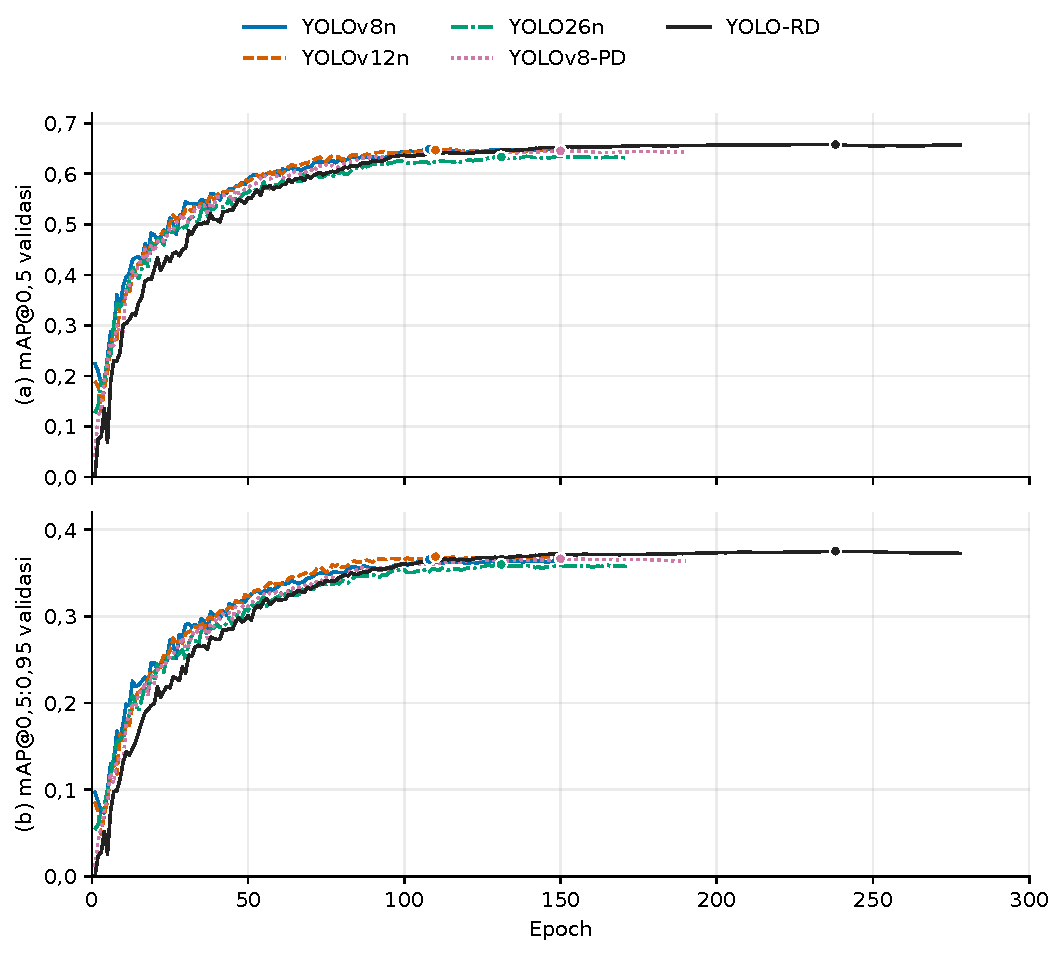
\includegraphics[width=\linewidth]{bab4-kurva-validasi.pdf}
\caption{Perkembangan mAP validasi pada pelatihan enam kelas. Titik menandai epoch terbaik berdasarkan mAP@0,5:0,95 validasi.}
\label{fig:b4-kurva}
\end{figure}
Gambar~\ref{fig:b4-kurva} memperlihatkan peningkatan metrik yang lebih besar pada bagian awal pelatihan, kemudian perubahan yang semakin kecil menjelang akhir. Model rekonstruksi memulai pelatihan dengan nilai validasi yang lebih rendah dan mencapai epoch terbaik lebih lambat. Kurva ini digunakan untuk menjelaskan proses pemilihan bobot, bukan menggantikan hasil pengujian akhir atau membuktikan terjadinya \textit{overfitting}.

\subsection{Kinerja deteksi pada data uji sumber}
Hasil agregat enam kelas disajikan pada Tabel~\ref{tab:b4-sumber}. Semua metrik dinyatakan pada skala nol sampai satu. Presisi dan \textit{recall} merupakan rata-rata kelas dari evaluator. F1 makro dirata-ratakan setelah F1 setiap kelas dihitung, bukan dari rata-rata presisi dan \textit{recall}.
% Generated by scripts/paper/thesis_bab4_assets.py; see build/bab4-qa/evidence.json.
\begin{table}[H]
\centering
\caption{Hasil pengujian sumber pada enam kelas.}
\label{tab:b4-sumber}
\begingroup\fontsize{10}{13}\selectfont
\setlength{\tabcolsep}{3pt}
\begin{tabularx}{\linewidth}{|X|r|r|r|r|r|}\hline
\rowcolor{black}\HeaderTabel{Model}&\HeaderTabel{Presisi}&\HeaderTabel{Recall}&\HeaderTabel{mAP@0,5}&\HeaderTabel{mAP@0,5:0,95}&\HeaderTabel{F1 makro}\\\hline
YOLOv8n & 0,643 & 0,599 & 0,648 & 0,364 & 0,617\\\hline
YOLOv12n & 0,638 & 0,608 & 0,654 & 0,371 & 0,619\\\hline
YOLO26n & 0,642 & 0,580 & 0,625 & 0,358 & 0,606\\\hline
YOLOv8-PD & 0,675 & 0,591 & 0,646 & 0,362 & 0,627\\\hline
YOLO-RD & 0,655 & 0,618 & 0,661 & 0,371 & 0,633\\\hline
\end{tabularx}\endgroup
\end{table}

Tabel~\ref{tab:b4-sumber} menunjukkan bahwa YOLO-RD memperoleh mAP@0,5 tertinggi sebesar 0,661 serta F1 makro tertinggi sebesar 0,633. YOLOv12n memperoleh mAP@0,5 sebesar 0,654. Pada mAP@0,5:0,95, kedua model bernilai 0,371 setelah pembulatan tiga desimal. YOLOv8-PD memiliki presisi tertinggi sebesar 0,675, sedangkan \textit{recall} tertinggi diperoleh YOLO-RD sebesar 0,618.

Rincian AP disajikan pada Tabel~\ref{tab:b4-kelas-sumber}. Identitas D00, D10, D20, D40, D70, dan D80 masing-masing merujuk pada retak memanjang, retak melintang, retak buaya, lubang, penutup saluran, dan jalan bertambal.
% Generated by scripts/paper/thesis_bab4_assets.py; see build/bab4-qa/evidence.json.
\begin{table}[H]
\centering
\caption{AP@0,5 per kelas pada data uji sumber.}
\label{tab:b4-kelas-sumber}
\begingroup\fontsize{10}{13}\selectfont
\setlength{\tabcolsep}{3pt}
\begin{tabularx}{\linewidth}{|X|r|r|r|r|r|r|}\hline
\rowcolor{black}\HeaderTabel{Model}&\HeaderTabel{D00}&\HeaderTabel{D10}&\HeaderTabel{D20}&\HeaderTabel{D40}&\HeaderTabel{D70}&\HeaderTabel{D80}\\\hline
YOLOv8n & 0,664 & 0,599 & 0,700 & 0,526 & 0,825 & 0,571\\\hline
YOLOv12n & 0,680 & 0,582 & 0,708 & 0,535 & 0,833 & 0,587\\\hline
YOLO26n & 0,639 & 0,567 & 0,675 & 0,538 & 0,820 & 0,512\\\hline
YOLOv8-PD & 0,678 & 0,572 & 0,702 & 0,541 & 0,819 & 0,562\\\hline
YOLO-RD & 0,696 & 0,608 & 0,701 & 0,527 & 0,845 & 0,587\\\hline
\end{tabularx}\endgroup
\end{table}

Tabel~\ref{tab:b4-kelas-sumber} menunjukkan bahwa penutup saluran memiliki AP@0,5 tertinggi pada setiap model, dengan rentang 0,819--0,845. Pada kelas lubang, nilainya berkisar 0,526--0,541. YOLOv8-PD mencapai AP lubang tertinggi, meskipun bukan pemilik mAP enam kelas tertinggi. Hasil ini memperlihatkan bahwa urutan model berdasarkan rata-rata tidak selalu sama dengan urutan pada satu kategori.

\subsection{Kompleksitas dan kecepatan pemrosesan}
Tabel~\ref{tab:b4-efisiensi} menyajikan kompleksitas model \textit{fused} pada masukan 640 piksel serta estimasi FPS sumber. Kompleksitas mengikuti penghitungan ulang \textit{checkpoint} akhir dengan Ultralytics 8.4.177. FPS mengikuti hasil validator pada RTX 4070 SUPER dan lingkungan pada Tabel~\ref{tab:lingkungan}.
% Generated by scripts/paper/thesis_bab4_assets.py; see build/bab4-qa/evidence.json.
\begin{table}[H]
\centering
\caption{Kompleksitas dan estimasi kecepatan model enam kelas.}
\label{tab:b4-efisiensi}
\begingroup\fontsize{10}{13}\selectfont
\setlength{\tabcolsep}{3pt}
\begin{tabularx}{\linewidth}{|X|r|r|r|}\hline
\rowcolor{black}\HeaderTabel{Model}&\HeaderTabel{Parameter (juta)}&\HeaderTabel{GFLOPs}&\HeaderTabel{FPS estimasi}\\\hline
YOLOv8n & 3,01 & 8,1 & 219,7\\\hline
YOLOv12n & 2,56 & 7,3 & 319,3\\\hline
YOLO26n & 2,38 & 5,3 & 293,3\\\hline
YOLOv8-PD & 2,47 & 7,7 & 368,4\\\hline
YOLO-RD & 7,09 & 12,8 & 189,4\\\hline
\end{tabularx}\endgroup
\end{table}

Tabel~\ref{tab:b4-efisiensi} memperlihatkan bahwa YOLO26n memiliki parameter dan GFLOPs paling rendah, masing-masing 2,38 juta dan 5,3. Estimasi FPS tertinggi diperoleh YOLOv8-PD sebesar 368,4, diikuti YOLOv12n sebesar 319,3. YOLO-RD memiliki parameter serta GFLOPs tertinggi dan estimasi FPS terendah pada pengukuran ini.

FPS dihitung dari waktu prapemrosesan, inferensi, dan pascapemrosesan sebelum pembulatan. Karena itu, perhitungan ulang dari waktu milidetik yang telah dibulatkan pada log dapat menghasilkan sedikit perbedaan. Angka kecepatan eksperimen tambahan empat kelas tidak digabungkan dalam tabel ini karena sebagian evaluasinya menggunakan GPU dan versi perangkat lunak berbeda.

\subsection{Kinerja menurut negara sumber}
Perbandingan negara disajikan pada Tabel~\ref{tab:b4-negara}. Rata-rata dibatasi pada empat kelas kerusakan untuk menghindari pengaruh perbedaan keberadaan kelas pengecoh. India tidak memiliki anotasi jalan bertambal dan hanya memiliki satu anotasi penutup saluran pada data uji.
% Generated by scripts/paper/thesis_bab4_assets.py; see build/bab4-qa/evidence.json.
\begin{table}[H]
\centering
\caption{mAP@0,5 empat kelas kerusakan menurut negara sumber.}
\label{tab:b4-negara}
\begingroup\fontsize{10}{13}\selectfont
\setlength{\tabcolsep}{3pt}
\begin{tabularx}{\linewidth}{|X|r|r|r|}\hline
\rowcolor{black}\HeaderTabel{Model}&\HeaderTabel{Tiongkok}&\HeaderTabel{Jepang}&\HeaderTabel{India}\\\hline
YOLOv8n & 0,931 & 0,578 & 0,284\\\hline
YOLOv12n & 0,933 & 0,579 & 0,293\\\hline
YOLO26n & 0,933 & 0,543 & 0,305\\\hline
YOLOv8-PD & 0,953 & 0,567 & 0,299\\\hline
YOLO-RD & 0,945 & 0,587 & 0,304\\\hline
\end{tabularx}\endgroup
\end{table}

Tabel~\ref{tab:b4-negara} menunjukkan pola yang sama pada seluruh model: nilai tertinggi terdapat pada subset Tiongkok, disusul Jepang dan India. YOLOv8-PD mencapai nilai tertinggi pada Tiongkok sebesar 0,953. Pada Jepang, nilai tertinggi diperoleh YOLO-RD sebesar 0,587. YOLO26n memperoleh nilai tertinggi pada India sebesar 0,305, meskipun perbedaannya dengan YOLO-RD kecil pada pembulatan yang digunakan.

Nilai gabungan sumber bukan rata-rata sederhana dari ketiga kolom tersebut. Evaluasi gabungan menghitung AP pada prediksi dan anotasi seluruh citra uji. Evaluasi per negara menghitung ulang AP pada masing-masing subset, yang memiliki komposisi citra dan objek berbeda.

\subsection{Hasil perbandingan konfigurasi label}
Hasil skenario kedua dirangkum pada Tabel~\ref{tab:b4-ablasi}. Kolom mAP 6 dan mAP 4 menyatakan mAP@0,5 empat kelas kerusakan dari model yang dilatih pada enam dan empat kelas. Kolom $\Delta$ mAP merupakan nilai empat kelas dikurangi nilai enam kelas. Kolom kotak menyatakan jumlah prediksi lubang yang bertumpang tindih dengan anotasi pengecoh.
% Generated by scripts/paper/thesis_bab4_assets.py; see build/bab4-qa/evidence.json.
\begin{table}[H]
\centering
\caption{Perbandingan pelatihan enam dan empat kelas pada data uji sumber.}
\label{tab:b4-ablasi}
\begingroup\fontsize{10}{13}\selectfont
\setlength{\tabcolsep}{3pt}
\begin{tabularx}{\linewidth}{|X|r|r|r|r|r|}\hline
\rowcolor{black}\HeaderTabel{Model}&\HeaderTabel{mAP 6}&\HeaderTabel{mAP 4}&\HeaderTabel{$\Delta$ mAP}&\HeaderTabel{Kotak 6}&\HeaderTabel{Kotak 4}\\\hline
YOLOv8n & 0,6224 & 0,6311 & +0,0088 & 3 & 3\\\hline
YOLOv12n & 0,6264 & 0,6280 & +0,0017 & 2 & 3\\\hline
YOLO26n & 0,6044 & 0,6036 & -0,0008 & 1 & 2\\\hline
YOLOv8-PD & 0,6233 & 0,6341 & +0,0108 & 2 & 2\\\hline
YOLO-RD & 0,6331 & 0,6511 & +0,0180 & 3 & 2\\\hline
\end{tabularx}\endgroup
\end{table}

Tabel~\ref{tab:b4-ablasi} menunjukkan peningkatan mAP pada empat pasangan model setelah label pengecoh dihapus, sedangkan YOLO26n mengalami penurunan 0,0008. Perubahan terbesar terdapat pada YOLO-RD, dari 0,6331 menjadi 0,6511. Selisih dihitung sebelum pembulatan, sehingga pengurangan angka tampilan dapat berbeda pada digit terakhir.

Pada pemeriksaan tumpang tindih, setiap konfigurasi menghasilkan satu sampai tiga kotak prediksi lubang. Seluruh kotak yang memenuhi kriteria bertumpang tindih dengan penutup saluran; tidak ada yang memenuhi kriteria pada jalan bertambal. Perbedaan pasangan konfigurasi adalah nol atau satu kotak. Hasil ini tidak menunjukkan pola penurunan yang konsisten ketika kelas pengecoh ditambahkan.

\subsection{Hasil pengujian pada target Indonesia}
\label{subsec:b4-target}
Perbandingan utama lintas domain disajikan pada Tabel~\ref{tab:b4-transfer}. Bobot yang digunakan tetap berasal dari pelatihan enam kelas. Kolom sumber dan target hanya merata-ratakan AP D00, D10, D20, dan D40. Kolom selisih menggunakan satuan poin persentase (pp), sedangkan kolom turun menggunakan persentase relatif terhadap sumber.
% Generated by scripts/paper/thesis_bab4_assets.py; see build/bab4-qa/evidence.json.
\begin{table}[H]
\centering
\caption{Perbandingan mAP@0,5 empat kelas kerusakan pada sumber dan target.}
\label{tab:b4-transfer}
\begingroup\fontsize{10}{13}\selectfont
\setlength{\tabcolsep}{3pt}
\begin{tabularx}{\linewidth}{|X|r|r|r|r|}\hline
\rowcolor{black}\HeaderTabel{Model}&\HeaderTabel{Sumber}&\HeaderTabel{Target}&\HeaderTabel{Selisih (pp)}&\HeaderTabel{Turun (\%)}\\\hline
YOLOv8n & 0,622 & 0,303 & 31,98 & 51,4\\\hline
YOLOv12n & 0,626 & 0,413 & 21,38 & 34,1\\\hline
YOLO26n & 0,604 & 0,301 & 30,32 & 50,2\\\hline
YOLOv8-PD & 0,623 & 0,342 & 28,18 & 45,2\\\hline
YOLO-RD & 0,633 & 0,359 & 27,45 & 43,4\\\hline
\end{tabularx}\endgroup
\end{table}

Tabel~\ref{tab:b4-transfer} menunjukkan penurunan pada seluruh model. YOLOv12n memperoleh mAP target tertinggi sebesar 0,413 dan penurunan relatif terkecil sebesar 34,1\%. YOLO-RD berada pada urutan kedua di target dengan mAP 0,359, meskipun memiliki nilai sumber tertinggi. Dengan demikian, peringkat kinerja berubah setelah model diterapkan pada data target lokal.

Rincian AP target disajikan pada Tabel~\ref{tab:b4-kelas-target}. D80 ditampilkan untuk kelengkapan pembahasan permukaan jalan, tetapi tidak masuk rata-rata empat kelas pada Tabel~\ref{tab:b4-transfer}. Jumlah anotasi D00, D10, D20, D40, dan D80 masing-masing adalah 231, 132, 48, 70, dan 21.
% Generated by scripts/paper/thesis_bab4_assets.py; see build/bab4-qa/evidence.json.
\begin{table}[H]
\centering
\caption{AP@0,5 per kelas pada data target Indonesia.}
\label{tab:b4-kelas-target}
\begingroup\fontsize{10}{13}\selectfont
\setlength{\tabcolsep}{3pt}
\begin{tabularx}{\linewidth}{|X|r|r|r|r|r|}\hline
\rowcolor{black}\HeaderTabel{Model}&\HeaderTabel{D00}&\HeaderTabel{D10}&\HeaderTabel{D20}&\HeaderTabel{D40}&\HeaderTabel{D80}\\\hline
YOLOv8n & 0,525 & 0,214 & 0,352 & 0,119 & 0,057\\\hline
YOLOv12n & 0,629 & 0,256 & 0,506 & 0,260 & 0,036\\\hline
YOLO26n & 0,534 & 0,157 & 0,296 & 0,218 & 0,039\\\hline
YOLOv8-PD & 0,558 & 0,217 & 0,442 & 0,149 & 0,062\\\hline
YOLO-RD & 0,585 & 0,275 & 0,468 & 0,107 & 0,075\\\hline
\end{tabularx}\endgroup
\end{table}

Tabel~\ref{tab:b4-kelas-target} memperlihatkan bahwa YOLOv12n memperoleh AP tertinggi pada retak memanjang, retak buaya, dan lubang. Pada retak melintang, YOLO-RD memperoleh nilai tertinggi sebesar 0,275. Lubang menjadi kategori dengan AP rendah pada semua model, dengan rentang 0,107--0,260. Nilai jalan bertambal lebih rendah lagi, yaitu 0,036--0,075, pada jumlah anotasi target yang lebih sedikit.

Evaluasi tambahan lima kelas disajikan pada Tabel~\ref{tab:b4-lima-kelas}. Kedua domain menggunakan D00, D10, D20, D40, dan D80 agar himpunan kelas tetap sebanding.
% Generated by scripts/paper/thesis_bab4_assets.py; see build/bab4-qa/evidence.json.
\begin{table}[H]
\centering
\caption{Evaluasi tambahan mAP@0,5 pada lima kelas bersama.}
\label{tab:b4-lima-kelas}
\begingroup\fontsize{10}{13}\selectfont
\setlength{\tabcolsep}{3pt}
\begin{tabularx}{\linewidth}{|X|r|r|r|}\hline
\rowcolor{black}\HeaderTabel{Model}&\HeaderTabel{Sumber}&\HeaderTabel{Target}&\HeaderTabel{Turun (\%)}\\\hline
YOLOv8n & 0,612 & 0,253 & 58,6\\\hline
YOLOv12n & 0,618 & 0,337 & 45,4\\\hline
YOLO26n & 0,586 & 0,249 & 57,5\\\hline
YOLOv8-PD & 0,611 & 0,286 & 53,3\\\hline
YOLO-RD & 0,624 & 0,302 & 51,6\\\hline
\end{tabularx}\endgroup
\end{table}

Tabel~\ref{tab:b4-lima-kelas} menunjukkan bahwa penyertaan jalan bertambal menurunkan rata-rata target pada seluruh model. YOLOv12n tetap berada pada urutan pertama dengan mAP 0,337 dan penurunan relatif 45,4\%. Angka tersebut merupakan hasil lima kelas, sehingga tidak menggantikan mAP empat kelas sebesar 0,413. Pemisahan kedua hasil menjaga konsistensi antara definisi metrik dan kesimpulan lintas domain.

\section{Analisis}
\subsection{Kinerja sumber dan perkembangan pelatihan}
Hasil sumber menunjukkan keunggulan teramati YOLO-RD pada metrik agregat, tetapi keunggulan itu tidak berlaku pada semua kelas. AP lubangnya sebesar 0,527 lebih rendah daripada YOLOv8-PD sebesar 0,541. Oleh sebab itu, pemilihan model berdasarkan mAP enam kelas perlu disertai pemeriksaan kategori yang diprioritaskan. Untuk tugas yang khusus berfokus pada lubang, peringkat agregat saja belum memadai.

Perbedaan mAP@0,5 dan mAP@0,5:0,95 juga menunjukkan pentingnya ketepatan lokasi kotak. Pada YOLO-RD, nilainya turun dari 0,661 menjadi 0,371 ketika digunakan rentang ambang IoU yang lebih ketat. Hasil ini memperlihatkan bahwa deteksi yang memenuhi ambang 0,5 belum selalu memenuhi ambang pencocokan lebih tinggi. Namun, kedua metrik tersebut tidak mengidentifikasi penyebab setiap kesalahan lokasi tanpa pemeriksaan prediksi lebih lanjut.

AP penutup saluran yang relatif tinggi tidak otomatis membuktikan keberhasilan label pengecoh dalam meningkatkan deteksi kerusakan. AP tersebut mengukur pengenalan kelas penutup saluran itu sendiri. Pengaruh konfigurasi label terhadap empat kelas kerusakan harus dibaca melalui pasangan eksperimen pada Tabel~\ref{tab:b4-ablasi}. Demikian pula, jumlah anotasi jalan bertambal yang sedikit merupakan konteks pembacaan hasil, bukan bukti bahwa ketimpangan menjadi satu-satunya penyebab AP rendah.

Kurva pada Gambar~\ref{fig:b4-kurva} melengkapi hasil uji dengan menunjukkan perbedaan perkembangan validasi. Epoch terbaik YOLO-RD yang lebih lambat disertai durasi pelatihan lebih panjang. Akan tetapi, durasi dipengaruhi pula oleh jumlah epoch, kompleksitas, pengaturan AMP, dan inisialisasi bobot. Ketiga model bawaan menggunakan AMP, sedangkan kedua rekonstruksi menonaktifkannya pada pelatihan utama.

Kedua rekonstruksi juga hanya memuat bagian bobot pralatih YOLOv8n yang kompatibel. Perbedaan ini dapat dipertimbangkan ketika membaca kurva awal dan biaya pelatihan, tetapi kontribusinya tidak diisolasi dalam eksperimen. Durasi lebih panjang tidak dapat ditafsirkan sebagai bukti bahwa suatu model belajar lebih baik atau memiliki generalisasi lebih kuat. Seluruh hasil merupakan pengamatan satu \textit{seed}, sehingga selisih kecil belum dinyatakan sebagai keunggulan yang konsisten pada pengulangan.

\subsection{Keseimbangan ketepatan dan kebutuhan komputasi}
Perbandingan Tabel~\ref{tab:b4-sumber} dengan Tabel~\ref{tab:b4-efisiensi} memperlihatkan beberapa pilihan sesuai prioritas penggunaan. YOLO-RD memberikan mAP sumber tertinggi, dengan kebutuhan parameter dan operasi terbesar. Dibandingkan YOLOv8n, selisih mAP@0,5 yang ditampilkan adalah sekitar 0,013. Peningkatan tersebut disertai pertambahan parameter dari 3,01 menjadi 7,09 juta dan penurunan estimasi FPS dari 219,7 menjadi 189,4.

YOLOv8-PD menggunakan parameter lebih sedikit daripada YOLOv8n dan memberikan estimasi FPS tertinggi, dengan mAP sumber yang berdekatan. Hasil ini sejalan dengan orientasi efisiensi rancangan YOLOv8-PD~\cite{Zeng2024}, tetapi bukan verifikasi kesamaan hasil dengan publikasi asal. Model yang diuji merupakan rekonstruksi lokal dengan transfer bobot parsial. Nilai AP tidak dibandingkan langsung dengan penelitian lain yang memakai data serta protokol berbeda.

YOLO26n memiliki GFLOPs paling rendah, tetapi tidak menghasilkan FPS tertinggi. Temuan ini menunjukkan bahwa estimasi jumlah operasi tidak dapat menggantikan pengukuran waktu pada perangkat tertentu. Perbandingan yang tersedia tidak memisahkan waktu setiap modul atau penyebab perbedaan pemanfaatan GPU. Dengan demikian, hasilnya cukup untuk mendeskripsikan hubungan kompleksitas dan kecepatan teramati, tanpa mengatribusikannya pada satu komponen arsitektur.

YOLOv12n menempati posisi yang relevan ketika ketepatan sumber, kecepatan, dan hasil target dipertimbangkan bersama. Model ini menghasilkan mAP sumber 0,654, estimasi 319,3 FPS, serta mAP target empat kelas tertinggi. Namun, tidak dibentuk skor gabungan untuk menyatakan satu model paling baik pada semua kebutuhan. Pemilihan kandidat tetap bergantung pada kategori, data sasaran, dan keterbatasan perangkat yang digunakan.

\subsection{Variasi sumber dan peran kelas pengecoh}
Pola antarnegera pada Tabel~\ref{tab:b4-negara} menunjukkan bahwa nilai gabungan sumber belum menjelaskan seluruh variasi kinerja. Semua model memperoleh nilai yang lebih rendah pada India daripada pada Tiongkok. Jumlah data latih Jepang juga lebih banyak daripada Tiongkok, tetapi tidak disertai nilai uji yang lebih tinggi. Karena komposisi objek serta karakteristik citra berbeda, hasil ini tidak mengisolasi pengaruh jumlah data latih.

Pembacaan per kelas pada subset kecil memerlukan kehati-hatian. Retak melintang pada India memiliki 19 anotasi latih dan enam anotasi uji. Jumlah tersebut membatasi kekuatan penilaian khusus kategori itu. Penggunaan empat kelas bersama menghilangkan perbedaan himpunan kategori dalam rata-rata, tetapi tidak menyamakan komposisi adegan atau tingkat kesulitan antarsubset.

Perbandingan label tidak memperlihatkan manfaat yang konsisten dari penambahan D70 dan D80 bagi mAP empat kelas kerusakan. Empat model justru memperoleh nilai lebih tinggi setelah anotasi pengecoh dihapus. Hasil ini menjawab dugaan yang mendasari penelitian pada kondisi eksperimen yang digunakan, tanpa menyimpulkan bahwa anotasi pengecoh selalu tidak bermanfaat.

Hitungan tumpang tindih memberikan informasi yang lebih terbatas daripada evaluasi AP. Selisih nol atau satu kotak antarpasangan belum memberikan bukti kuat tentang perubahan kesalahan deteksi. Tidak ditemukannya tumpang tindih pada jalan bertambal hanya berlaku pada ambang yang ditetapkan. Hasil tersebut tidak berarti bahwa seluruh prediksi lubang benar atau bahwa tidak ada kebingungan pada ambang lain.

Penghilangan label juga mengubah pembobotan kelas dan tugas klasifikasi yang dipelajari. Selain itu, AMP pada kedua model rekonstruksi berbeda antara pelatihan utama dan eksperimen empat kelas. Karena itu, perubahan skor dibaca sebagai hasil perbandingan konfigurasi lengkap. Eksperimen ini belum memisahkan pengaruh label pengecoh dari seluruh faktor pelatihan lainnya secara kausal.

\subsection{Generalisasi dan contoh kesalahan pada target}
Perubahan peringkat sumber dan target menunjukkan bahwa pemilihan model hanya dari mAP sumber tidak cukup untuk menentukan kandidat terbaik pada citra jalan lokal. YOLO-RD memimpin evaluasi sumber, sedangkan YOLOv12n memimpin evaluasi target empat kelas. Meskipun demikian, YOLOv12n masih mengalami penurunan relatif sebesar 34,1\%. Keunggulannya bersifat relatif terhadap model pembanding pada target yang diuji, bukan bukti bahwa persoalan transfer domain telah terselesaikan.

Perbandingan per kelas memperjelas ruang perbaikan. YOLOv12n mempertahankan AP retak memanjang sebesar 0,629 pada target, sedangkan AP lubangnya hanya 0,260. Model tersebut juga belum kuat pada jalan bertambal, dengan AP 0,036. Hasil ini menegaskan bahwa nilai rata-rata target yang lebih tinggi tidak menjamin seluruh jenis cacat permukaan dikenali dengan baik.

Contoh visual pada Gambar~\ref{fig:b4-target} digunakan untuk menelaah bentuk kesalahan yang menyertai hasil kuantitatif. Gambar diambil dari visualisasi eksperimen target yang sama dengan paper. Kolom memperlihatkan anotasi acuan dan prediksi tiga model, sedangkan setiap baris menunjukkan satu citra.
\begin{figure}[H]
\centering
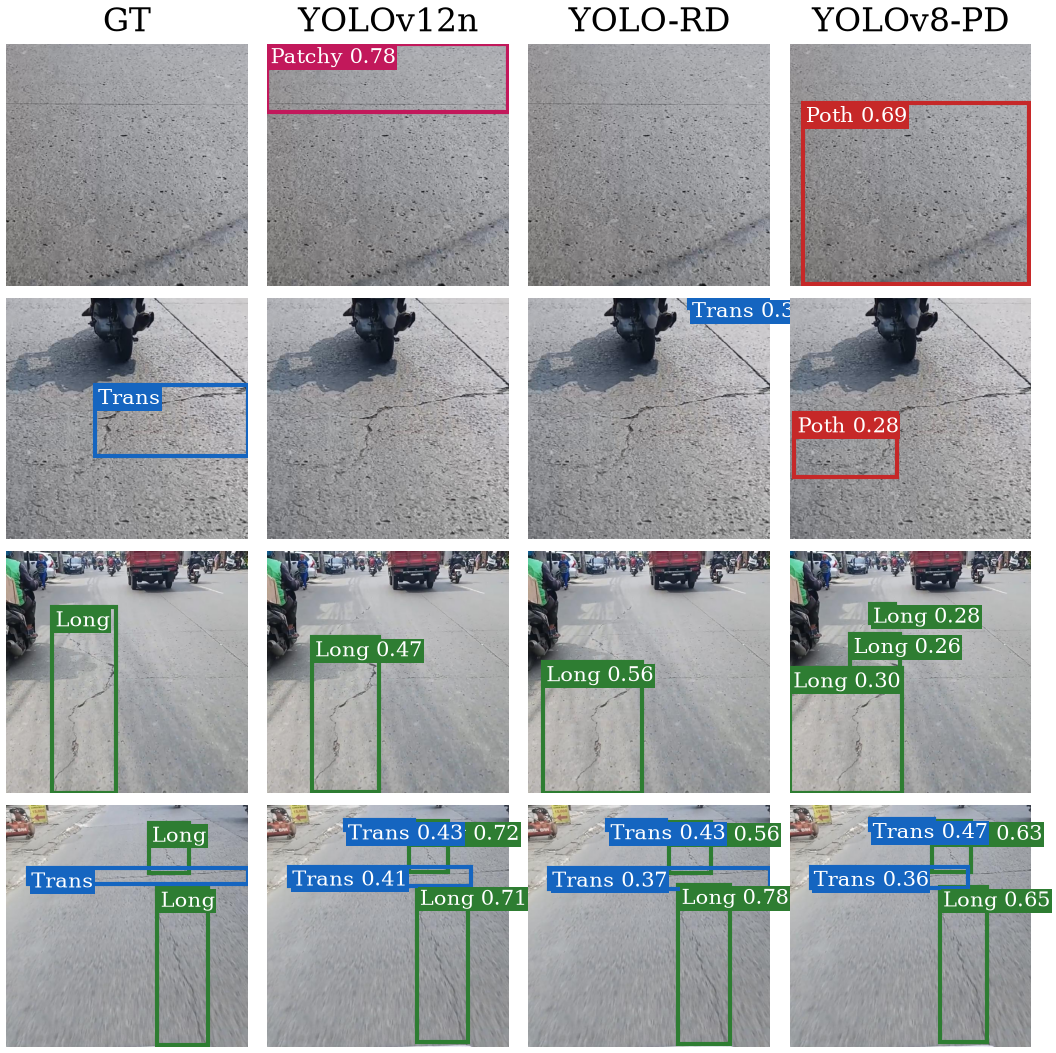
\includegraphics[width=\linewidth]{bab4-contoh-target.png}
\caption{Anotasi acuan dan prediksi pada empat citra target terpilih. Urutan kolom: GT, YOLOv12n, YOLO-RD, dan YOLOv8-PD; ambang tampilan 0,25.}
\label{fig:b4-target}
\end{figure}
Gambar~\ref{fig:b4-target} menampilkan dua contoh dengan kesalahan yang menonjol serta dua contoh dengan retak yang terdeteksi. Singkatan Long, Trans, Poth, dan Patchy pada kotak masing-masing menunjukkan retak memanjang, retak melintang, lubang, dan jalan bertambal. Prediksi tetap menampilkan kategori keluaran model enam kelas, sehingga label jalan bertambal dapat muncul meskipun tidak masuk metrik utama empat kelas.

Pada baris pertama, citra tidak memiliki anotasi kerusakan. YOLOv12n menghasilkan prediksi jalan bertambal dan YOLOv8-PD menghasilkan prediksi lubang, sedangkan YOLO-RD tidak menampilkan kotak pada ambang yang digunakan. Pada baris kedua, YOLOv12n melewatkan retak melintang beranotasi. YOLO-RD menghasilkan kotak retak melintang kecil dengan lokasi yang tidak sesuai, sedangkan YOLOv8-PD memprediksi lubang.

Pada baris ketiga, ketiga model mendeteksi retak memanjang, tetapi YOLOv8-PD menampilkan lebih dari satu kotak. Baris keempat memuat dua anotasi retak memanjang dan satu anotasi retak melintang. Prediksi menangkap retak tersebut, tetapi juga menampilkan kotak retak melintang tambahan. Contoh ini membantu membedakan objek terlewat, kekeliruan kategori, dan kotak tambahan; jumlah baris tidak mewakili frekuensi kesalahan pada seluruh target.

Perbedaan tampilan perkerasan, sudut pengambilan gambar, dan pencahayaan dapat menjadi konteks perubahan domain sebagaimana dibahas pada Bab~\ref{bab:tinjauan-pustaka}. Namun, eksperimen ini tidak mengubah faktor tersebut satu per satu. Penurunan mAP konsisten dengan adanya kesenjangan kinerja antardataset, tetapi tidak menentukan besarnya kontribusi tekstur, pencahayaan, atau lokasi. Kinerja transfer juga tidak dapat diatribusikan langsung kepada modul perhatian tanpa eksperimen yang mengisolasi modul itu.

\subsection{Keterkaitan hasil dan keterbatasan penelitian}
Rumusan masalah pertama dijawab melalui hasil agregat dan per kelas pada sumber, disertai perbandingan konfigurasi label. YOLO-RD menghasilkan mAP enam kelas tertinggi pada pengujian ini. Penambahan label pengecoh tidak menunjukkan manfaat yang konsisten terhadap empat kelas kerusakan ataupun jumlah tumpang tindih yang diperiksa. Kedua temuan tersebut perlu dipisahkan karena mengukur aspek yang berbeda.

Rumusan masalah kedua dijawab oleh perbandingan parameter, GFLOPs, dan estimasi FPS. YOLO26n paling kecil menurut parameter dan GFLOPs, sedangkan YOLOv8-PD memiliki estimasi FPS tertinggi. Rumusan masalah ketiga dijawab oleh penurunan kinerja seluruh model dan perubahan peringkat pada target. YOLOv12n memberikan hasil transfer tertinggi pada empat kelas kerusakan yang sama.

Kekuatan kesimpulan dibatasi oleh satu \textit{seed}, perbedaan kapasitas, transfer bobot pralatih, AMP, dan implementasi rekonstruksi. Pengaturan otomatis optimizer juga tidak menjamin seluruh model memiliki konfigurasi efektif identik. Oleh sebab itu, perbedaan skor tidak dinyatakan signifikan secara statistik dan tidak diperlakukan sebagai pengaruh murni satu komponen arsitektur.

Data target mencakup lokasi terbatas di Kabupaten Bandung dan dianotasi oleh satu orang tanpa pengukuran kesepakatan antar-anotator. Citra berasal dari video, sedangkan tingkat kemiripan antarbingkai belum diukur dalam analisis ini. Hasil pada 307 citra tersebut tidak digeneralisasi sebagai kinerja seluruh jalan Indonesia. Evaluasi yang lebih luas diperlukan untuk menilai kestabilan peringkat pada lokasi dan kondisi perekaman lain.

F1 yang dilaporkan mengikuti titik operasi hasil optimasi kurva pada bagian data yang dievaluasi. Nilainya tidak mewakili ambang penerapan yang telah ditetapkan dari validasi sumber. Estimasi FPS juga berasal dari validator pada GPU desktop, bukan pengujian aplikasi jalan secara langsung. Batas-batas ini menjadi dasar penarikan kesimpulan dan saran pengembangan pada bab berikutnya.

\chapter{KESIMPULAN DAN SARAN}

\label{bab:kesimpulan-dan-saran}

\section{Kesimpulan}

Bab ini memuat elaborasi dan rincian simpulan yang kemudian menjadi bagian abstraks. Simpulan ditarik dari hasil analisis secara komprehensif atas eksperimen yang telah dilakukan dan dinyatakan dalam bentuk narasi satu dua paragraf. Dalam Simpulan menggambarkan tingkat ketercapaian atas Tujuan Tugas Akhir yang telah dinyatakan dalam Bab 1.

\section{Saran}

Di dalam Saran, untuk pengembangan penelitian sebelumnya, pembuatan sistem disarankan untuk lebih xxx, sehingga tujuan dapat lebih tercapai. Alasannya :

\begin{enumerate}[series=word32level0,label=\alph*.]

\item Harus lebih mengidentifikasi masalah.

\item Harus menyesuaikan dengan teknologi yang ada.

\item Kelemahan-kelemahan yang terjadi.

\end{enumerate}

\clearpage
\phantomsection\addcontentsline{toc}{chapter}{DAFTAR PUSTAKA}
\begingroup
\referencefont\fontsize{10}{12}\selectfont
\setlength{\bibsep}{3pt}
\bibliographystyle{IEEEtran}
\bibliography{References}
\endgroup
\HalamanAwal{LAMPIRAN}
Lampiran dapat berisi kode sumber, tabel-tabel yang diperlukan dalam penelitian tetapi kurang relevan untuk dimasukkan dalam bab-bab Tugas Akhir.

% Tambahkan lampiran di sini; contoh judul: \section*{Lampiran A. Kode Sumber}

\end{document}
